\section{Conditional convergence in the multiphase case}

\subsection{Convergence to a $\bv$-solution for multiphase mean curvature flow}

We start by defining a $ \bv $-formulation for motion by multiphase mean 
curvature flow under the simplifying assumption that the mobilities are already 
fixed by the surface tensions through the equation
\begin{equation}
	\label{mobilites_inverse_of_surface_tensions}
	\mu_{ i j } =\frac{ 1 }{ \sigma_{ i j } }. 
\end{equation}
Note moreover that in this section, all expressions refer to their multiphase 
equivalent.

\begin{definition}[$\bv$-solution to multiphase mean curvature flow]
	\label{motion_by_mmcf}
	Fix some finite time horizon $ T < \infty $, a $ P \times P $ matrix of 
	surface tensions $ \sigma $ and initial data $ \chi^{ 0 } \colon \flattorus 
	\to \{ 0 , 1 \}^{ P } $ with $ \energy_{ 0 } \coloneqq \energy ( \chi^{ 0 } 
	) < \infty $ and 
	$ \sum_{ i = 1 }^{ P } \chi_{ i }^{ 0 } = 1 $. We say that
	\begin{equation*}
		\chi \in \cont \left(
		[ 0 , T ]
		;
		\lp^{ 2 } \left( \flattorus ; \{ 0 , 1 \}^{ P } \right)
		\right)
	\end{equation*}
	with $ \esssup_{ 0 \leq t \leq T } \energy ( \chi ) $ and $ \sum_{ i = 1 
	}^{ P } \chi_{ i } = 1 $ \emph{moves by mean curvature with initial data} $ 
	\chi^{ 0 } $ \emph{and surface tensions} $ \sigma $ if there exist normal 
	velocities $ V_{ i } \in \lp^{ 2 } ( \abs{ \nabla \chi_{ i } } \dd{ t } ) $ 
	with
	\begin{equation*}
		\int_{ 0 }^{ T }
		\int
		V_{ i }^{ 2 }
		\abs{ \nabla \chi_{ i } }
		\dd{ t }
		< \infty 
	\end{equation*} 
	such that
	\begin{enumerate}
		\item For all 
		$ \xi \in \cont_{ \mathrm{c} }^{ \infty } \left(
		( 0 , T ) \times \flattorus ; \mathbb{ R }^{ d }
		\right)
		$, we have 
		\begin{align}
			\label{distributional_equation_mmcf}
			\sum_{ 1 \leq i < j \leq P }
			\sigma_{ i j }
			\int_{ 0 }^{ T }
			\int
			&
			\left(
			V_{ i } \inner*{ \xi }{ \nu_{ i } }
			-
			\inner*{ \diff \xi }{ \mathrm{Id} - \nu_{ i } \otimes \nu_{ i } }
			\right)
			\times
			\\
			\notag
			& \frac{1}{ 2 }
			\left(
			\abs{ \nabla \chi_{ i } }
			+
			\abs{ \nabla \chi_{ j } }
			-
			\abs{ \nabla ( \chi_{ i } + \chi_{ j } ) }
			\right)
			\dd{ t }
			=0,			
		\end{align}
		where $ \nu_{ i } $ is the inner unit normal of $ \chi_{ i } $.
		
		\item 
		The functions $ V_{ i } $ are the normal velocities of the interfaces 
		in the sense that
		\begin{equation*}
			\partial_{ t } \chi_{ i }
			=
			V_{ i } \abs{ \nabla \chi_{ i } } \dd{ t }
		\end{equation*}
		holds distributionally on $ ( 0 , T ) \times \flattorus $.
		
		\item
		The initial data is achieved in the space $ \cont \left( [ 0 , T ] ; 
		\lp^{ 2 } ( \flattorus ) \right) $.
	\end{enumerate}
\end{definition}

Since (\ref{distributional_equation_mmcf}) is quite the long equation, we want 
to motivate it as a suitable weak formulation for multiphase mean curvature 
flow. 
Assuming that everything is nice and smooth, we have by the 
Gauss-Green theorem on surfaces 
\cite[Thm.~11.8]{maggi_sets_of_finite_perimeter} that
\begin{equation*}
	\int_{ \Sigma_{ i j } }
	\int 
	\inner{ \diff \xi }{ \mathrm{Id} - \nu \otimes \nu }
	\dd{\hm^{ d- 1 }}
	=
	-
	\int_{ \Sigma_{ i j } }
	\int
	H \inner*{ \xi }{ \nu }
	\dd{\hm^{ d- 1 }}
	+
	\int_{ \Gamma_{ i j } }
	\int
	\inner*{ \xi }{ \nu_{ \Gamma } }
	\dd{ \hm^{ d - 2 } }.
\end{equation*}
Here $ \Gamma_{ i j } $ denotes the boundary of the surface $ \Sigma_{ i j 
} $ and $ \nu_{ \Gamma } $ the corresponding unit normal. But then Herring's 
angle condition 
(\ref{herrings_angle_condition}) tells us that the boundary terms cancel 
out. In fact, Herring's angle condition does not contain the boundary unit 
normals $ \nu_{ \Gamma } $, but one can show that these are just the rotations 
of the regular unit normals of the surfaces, and that the rotation is 
independent of the chosen interface at the triple junction. Therefore equation 
(\ref{distributional_equation_mmcf}) is now the sum of integrals over
each interface of
\begin{equation*}
	(V_{ i } + H) \inner*{ \xi }{ \nu_{ i } },
\end{equation*}
which is zero by equation (\ref{v_is_equal_to_h}) combined with the 
assumption for the mobilities (\ref{mobilites_inverse_of_surface_tensions}).

Our main goal will be to arrive at a conditional convergence result 
to multiphase mean curvature flow in the sense of the above definition. 
This is captured by the following.

\begin{theorem}
	\label{convergence_to_multiphase_mcf}
	Let a smooth multiwell potential $ W \colon \mathbb{ R }^{ N } \to [ 0, 
	\infty ) $ satisfy the assumptions 
	(\ref{polynomial_growth})-(\ref{perturbation bound}). Let $ T < \infty 
	$ be an arbitrary finite time horizon. Given a sequence of initial data 
	$ u_{ \varepsilon }^{ 0 } \colon \flattorus \to \mathbb{ R }^{ N } $ 
	approximating a partition 
	$ \chi^{ 0 } \in \bv \left( \flattorus ; \{ 0 , 1 \}^{ P } \right) $ 
	in the sense that 
	$ u_{ \varepsilon }^{ 0 } \to u^{ 0 } =  \sum_{ 1 \leq i \leq P } 
	\chi_{ i }^{ 0 } \alpha_{ i } $ 
	holds pointwise almost everywhere and 
	\begin{equation*} 
		\energy_{ 0 } 
		\coloneqq 
		\energy ( \chi^{ 0 } ) 
		= 
		\lim_{ \varepsilon \to 0 } 
		\energy_{ \varepsilon } ( u_{ \varepsilon }^{ 0 } ) 
		< 
		\infty,
	\end{equation*}
	we have that for 
	some subsequence of solutions $ u_{\varepsilon } $ to the Allen--Cahn 
	equation
	(\ref{allen_cahn_eq}) with initial datum $ u_{ 
		\varepsilon }^{ 0 } $, there exists a time-dependent partition $ \chi $ 
	with 
	$ \chi \in \bv \left( ( 0 , T ) \times \flattorus ; \{ 0 , 1 \}^{ P } 
	\right) $ and
	$ \chi 
	\in \cont \left( [ 0 , T ] ; \lp^{ 2 } \left( \flattorus ;  \{ 0 , 1 
	\}^{ P } \right) \right) $ such that $ u_{ \varepsilon } $ converges to 
	$ u \coloneqq \sum_{ 1 \leq i \leq P } \chi_{ i } \alpha_{ i } $ almost 
	everywhere. Moreover $ u $ assumes the initial data $ u^{ 0 } $ in $ 
	\cont \left( [ 0, T ] ; \lp^{ 2 }( \flattorus ) \right) $. If we 
	additionally assume that the 
	time-integrated energies converge (\ref{energy_convergence}), then $ 
	\chi $ moves by mean curvature in the sense of \Cref{motion_by_mmcf}.
\end{theorem} 

First we are going to prove the existence of normal velocities $ V_{ 
i } $ for the evolving sets $ \Omega_{ i } $ under the assumption of the energy 
convergence
(\ref{energy_convergence}).

\begin{proposition}
	\label{existence_and_square_integrability_of_velocities_multiphase}
	In the situation of \Cref{initial_convergence_result_multiphase} and under 
	the energy convergence assumption (\ref{energy_convergence}), we have that 
	for every $ 1 \leq i \leq P $, the signed measure $ \partial_{ t } \chi_{ i 
	} $ is absolutely continuous with respect to the measure $ \abs{ \nabla 
	\chi_{i } } \dd{ t } $ and the corresponding density $ V_{ i } $ is square 
	integrable with the corresponding estimate
	\begin{equation}
		\label{velocity_l2_estimate}
		\int_{ 0 }^{ T }
		\int
		V_{ i }^{ 2 }
		\abs{ \nabla \chi_{ i } }
		\dd{ t }
		\lesssim
		\energy_{ 0 }.
	\end{equation}
\end{proposition}

\begin{proof}
	The proof proceeds in four steps. First we show that $ \partial_{ t } 
	\psi_{ i } $ is absolutely continuous with respect to the energy measure. 
	Afterwards, we show that we can already estimate $ \abs{ \partial_{ t } 
	\chi_{ i } } $ by $ \abs{ \partial_{ t } \psi_{ i } } $. To finish the 
	argument, we then we have to argue that $ \partial_{ t } \chi_{ i } $ is 
	already singular with respect to every part of the energy which is not 
	contained in $ \abs{ \nabla \chi_{ i } } \dd{ t } $.
	
	\begin{description}[wide=0pt]
		\item[Step 1:] The signed measure $ \partial_{  t } \psi_{ i } $ is 
		absolutely continuous with respect to the energy measure $ \energy ( 
		\cdot, u ) \dd{t } $ with square-integrable density.
		
		Let $ \varphi $ be a testfunction. Then we can estimate by 
		Hölder's inequality
		\begin{align*}
			\partial_{ t } \psi_{ i } ( \varphi )
			& =
			\liminf_{ \varepsilon \to 0 }
			\int_{ 0 }^{ T }
			\int
			\varphi
			\partial_{ t } \psi_{ \varepsilon ,i }
			\dd{ x }
			\dd{ t }
			\\
			& \leq
			\liminf_{ \varepsilon \to 0 }
			\left(
			\int_{ 0 }^{ T }
			\int
			\varepsilon 
			\abs{ \partial_{ t } u_{ \varepsilon } }^{ 2 }
			\dd{ x }
			\dd{ t }
			\right)^{ 1/2 }
			\left(
			\int_{ 0 }^{ T }
			\int
			\varphi^{ 2 }
			\frac{ 1 }{ \varepsilon }
			2 W ( u_{ \varepsilon } )
			\dd{ x }
			\dd{ t }
			\right)^{ 1/2 }
			\\
			& \leq
			\sqrt{ \energy_{ 0 } }
			\left(
			\int_{ 0 }^{ T }
			\energy ( u ; \varphi )
			\dd{ t }
			\right)^{ 1/2 }.
		\end{align*}
		Here the last inequality is due to the energy dissipation 
		(\ref{energy_dissipation_sharp})
		and the proof of our claim is therefore complete.
		
		\item[Step 2:] For $ d_{ i } \coloneqq \min_{ j \neq i } \sigma_{ i j } 
		$, we have 
		that $ d_{ i } \abs{ \partial_{ t } \chi_{ i } } \leq \abs{ \partial_{ 
		t } \psi_{ i } } $.
		
		Using the disintegration Theorem 
		\cite[Thm.~3.103]{ambrosio_fusco_pallara_functions_of_bv_and_free_discontinuity_problems}
		 and the Fleming--Rishel co-area formula, we have for any open set 
		$ U \subseteq ( 0 , T ) \times \flattorus $ that
		\begin{align*}
			\abs{
				\partial_{ t } \psi_{ i }
			} ( U ) 
			& =
			\int
			\abs{ 
				\partial_{ t } \psi_{ i } ( \cdot , x )
			} ( \pi_{ x } ( U ) ) 
			\dd{ x }
			\\
			& =
			\int
			\int_{ 0 }^{ \infty }
			\hm^{ 0 } \left(
			\left\{
			t 
			\, \colon \,
			\sum_{ j } \chi_{ j } \sigma_{ i j } > s,
			( t, x ) \in U
			\right\}
			\right)
			\dd{ s }
			\dd{ x }
			\\
			& \geq
			\int
			\int_{ 0 }^{ d_{ i } }
			\hm^{ 0 }
			\left(
			\left\{
			t 
			\, \colon \,
			\chi_{ i } ( t , x ) = 1,
			( t, x ) \in U
			\right\}
			\right)
			\dd{ s }
			\dd{ x }
			\\
			& =
			d_{ i }
			\int
			\int_{ 0 }^{ \infty }
			\hm^{ 0 } \left(
			\left\{
			t 
			\, \colon \,
			\chi_{ i } ( t , x ) > s , ( t , x ) \in U
			\right\}
			\right)
			\dd{ s }
			\dd{ x }
			\\
			& =
			d_{ i }
			\abs{ \partial_{ t } \chi_{ i } } ( U ).
		\end{align*}
		Here the set $ \pi_{ x } ( U ) $ denotes the set of all $ t $ such that 
		$ ( t , x ) $ is an element of $ U $. This completes the proof.
		
		\item[Step 3:] The signed measure $ \partial_{ t } \chi_{ i } $ is 
		singular to the wrong parts of $ \energy ( u ; \cdot ) $. More 
		precisely we claim that if $ 1 \leq j < k \leq P $ and $ i \notin \{ j 
		, k \} $, then the measures 
		$ \hm^{ d - 1 } |_{ \Sigma_{ j k } } \dd{ t } $ and $ \abs{ \partial_{ 
				t } \chi_{ i } } $ are mutually singular.
		
		We again write $ \abs{ \nabla \chi }_{ d + 1 } $ for the space 
		derivative in time and space and $ \abs{ \nabla \chi }_{ d } $ for the 
		space derivative for some fixed time $ t $, which is defined for almost 
		every time. Moreover, we denote by $ \tilde{ \Omega }_{ i } $ the set 
		in time and space such that
		$ \chi_{ i } ( t , x ) = \mathds{ 1 }_{ \tilde{ \Omega }_{ i } } ( t , 
		x ) $
		and by $ \tilde{ \Sigma }_{ i j } $ the corresponding interfaces.
		By \Cref{identities_for_measure_theoretic_boundaries} we can then write
		\begin{equation*}
			\abs{ \partial_{ t } \chi_{ i } }
			\leq
			\abs{ ( \partial_{ t } , \nabla ) \chi_{ i } }
			=
			\sum_{ l \neq i }
			\hm^{ d } |_{ \partial_{ \ast } \tilde{ \Omega }_{ i } \cap 
			\partial_{ \ast } \tilde{ \Omega }_{ l } }.
		\end{equation*}
		But for all $ l \neq i $, we have again by 
		\Cref{identities_for_measure_theoretic_boundaries} that either 
		\begin{equation*}
			\abs{ ( \partial_{ t } , \nabla ) \chi_{ j } } ( \tilde{ \Sigma }_{ 
				i l } ) = 0 
			\quad \text{or} \quad
			\abs{ ( \partial_{ t } , \nabla ) \chi_{ k } } ( \tilde{ \Sigma }_{ 
				i l } ) = 0.
		\end{equation*}
		Without loss of generality we assume the former. 
		Then it follows that $ \abs{ \nabla \chi_{ j } }_{ d + 1 } \left( 
		\tilde{ \Sigma }_{ i l } \right) = 0 $ and therefore we have
		\begin{align*}
			\hm^{ d - 1 } |_{ \Sigma_{ j k } } \dd{ t } ( \tilde{ \Sigma }_{ i 
				l } )
			& =
			\frac{ 1 }{ 2 } \left(
			\abs{ \nabla \chi_{ j } }_{ d }
			+
			\abs{ \nabla \chi_{ k } }_{ d }
			-
			\abs{ \nabla ( \chi_{ j } + \chi_{ k } ) }_{ d }
			\right)
			\dd{ t }
			\left( \tilde{ \Sigma }_{ i l }\right)
			\\
			& = 
			\frac{ 1 }{ 2 } \left(
			\abs{ \nabla \chi_{ j } }_{ d+1 }
			+
			\abs{ \nabla \chi_{ k } }_{ d +1 }
			-
			\abs{ \nabla ( \chi_{ j } + \chi_{ k } ) }_{ d+ 1 }
			\right) \left( \tilde{ \Sigma }_{ i l } \right)
			\\
			& = 
			\frac{ 1 }{ 2 } \left( 
			\abs{ \nabla \chi_{ k } }_{ d + 1 } \left( \tilde{ \Sigma } _{ i , 
			l } \right)
			-
			\abs{ \nabla \chi_{ k } }_{ d + 1 } 
			\left( \tilde{ \Sigma } _{ i l } \right)
			\right)
			= 0.		
		\end{align*}
		This proves the desired singularity.
		
		\item[Step 4:] We have 
		$ \abs{ \partial_{ t } \chi_{ i } } 
		\leq \abs{ \nabla \chi_{ i } } \dd{ t } $ and estimate 
		(\ref{velocity_l2_estimate}) holds.
		
		Combining Step 1 and Step 2, we obtain that $ \abs{ \partial_{ t } 
		\chi_{ i } } $ is absolutely continuous with respect to the energy 
		measure $ \energy ( u ; \cdot ) $. Moreover we can write
		\begin{equation*}
			\energy ( u ; \cdot ) \dd{ t }
			=
			\sum_{ j \neq i }
			\sigma_{ i j }
			\hm^{ d - 1 } |_{ \Sigma_{ i j } }
			\dd{ t }
			+
			\sum_{ 1 \leq j < k \leq P , j, k \neq i }
			\sigma_{ j k }
			\hm^{ d- 1 } |_{ \Sigma_{ j k } }
			\dd{ t }.
		\end{equation*}
		The second sum is by Step 3 singular to $ \abs{ 
		\partial_{ t } \chi_{ i } } $ and the first sum is bounded by $ 
		\abs{ \nabla \chi_{ i } } \dd{ t } $, which proves that $ \partial_{ t 
		} \chi_{ i } $ is absolutely continuous with respect to $ \abs{ \nabla 
		\chi_{ i } } \dd{ t } $.
		Lastly the desired estimate (\ref{velocity_l2_estimate}) is now a 
		consequence of our 
		previous arguments combined with a duality estimate. By Step 3 we find 
		a Borel-measurable set $ S $ such that for all $ j, k \neq i $, we have 
		$ \hm^{ d-  1 } |_{ \Sigma_{ j k } } \dd{ t } ( S ) = 0 $ and $ \abs{ 
		\partial_{ t } \chi_{ i } } ( ( 0 , T ) \times \flattorus \setminus S ) 
		= 0 $. Fix some $ K > 0 $ 
		and let $ \varphi_{ n } $ be a sequence of testfunctions which 
		converges in 
		$ \lp^{ 2 } \left( \abs{ \nabla \chi_{ i } } \dd{ t } \right) $ to the 
		function
		$ V_{ i } \mathds{ 1 }_{ \abs{ V_{ i } } \leq K } \mathds{ 1 }_{ 
		S } $. Then combining the 
		previous steps, we can estimate
		\begin{align*}
			\int_{ 0 }^{ T }
			\int
			V_{ i }^{ 2 } \mathds{ 1 }_{ \abs{ V_{ i } } \leq K }
			\abs{ \nabla \chi_{ i } }
			\dd{ t }
			& =
			\liminf_{ n \to \infty }
			\abs{
				\int_{ 0 }^{ T }
				\int
				V_{ i } \varphi_{ n } 
				\abs{ \nabla \chi_{ i } }
				\dd{ t }
			}
			\\
			& = 
			\liminf_{ n \to \infty }
			\abs{
				\int_{ 0 }^{ T }
				\int
				\varphi_{ n } \partial_{ t } \chi_{ i }
			}
			\\
			& \lesssim
			\liminf_{ n \to \infty }
			\int_{ 0 }^{ T }
			\int
			\varphi_{ n }^{ 2 }
			\abs{ \partial_{ t } \psi_{ i } }
			\\
			& \leq
			\sqrt{ \energy_{ 0 } }
			\liminf_{ n \to \infty }
			\left(
			\int_{ 0 }^{ T }
			\energy ( u ; \varphi_{ n }^{ 2 } )
			\dd{ t }
			\right)^{ 1/2 }
			\\
			& \lesssim
			\sqrt{ \energy_{ 0 } }
			\left(
			\int_{ 0 }^{ T }
			\int
			V_{ i }^{ 2 }
			\mathds{ 1 }_{ \abs{ V_{ i } } \leq K }
			\abs{ \nabla \chi_{ i } }
			\dd{ t }
			\right)^{ 1 / 2 }.
		\end{align*}
		This proves by the monotone convergence theorem the desired claim.
	\end{description} 
	Therefore our proof is complete.
\end{proof}

As in the twophase case \Cref{equipartition_of_energies}, we have an 
equipartition of energies. The proof is similar and therefore left out.

\begin{lemma}
	\label{equipartition_of_energies_multiphase}
	In the situation of \Cref{initial_convergence_result_multiphase} and under 
	the energy convergence assumption (\ref{energy_convergence}), we have for 
	any continuous $ \varphi \in \cont ( \flattorus ) $ that
	\begin{align*}
		\energy ( u ; \varphi )
		=
		\lim_{ \varepsilon \to 0 }
		\energy_{ \varepsilon } ( u_{ \varepsilon } ; \varphi )
		& =
		\lim_{ \varepsilon \to 0 }
		\int
		\varphi
		\varepsilon
		\abs{ \nabla u_{ \varepsilon } }^{ 2 }
		\dd{ x }
		\\
		& =
		\lim_{ \varepsilon \to 0 }
		\int
		\varphi
		\frac{ 1 }{ \varepsilon } 2 W ( u_{ \varepsilon } )
		\dd{ x }
		\\
		& =
		\lim_{ \varepsilon \to 0 }
		\int
		\varphi
		\sqrt{ 2 W ( u_{ \varepsilon } ) }
		\abs{ \nabla u_{ \varepsilon } }
		\dd{ x }
	\end{align*}
	for almost every time $ 0 \leq t \leq T $.
\end{lemma}

\subsection{Localization estimates}
\label{section_localization_estimates}
In order to prove convergence of the curvature and velocity term, we want to 
reduce the multiphase case to the two-phase case. The central idea here is to 
cover the flat torus with a suitable covering of balls and argue that, up to a 
small error, we can choose 
for each ball majority phases $ i, j $ such that the partition looks like a 
two-phase mean curvature flow on the ball, see 
\Cref{figure_localization_of_mmcf}.

\begin{figure}[h]
	\centering
	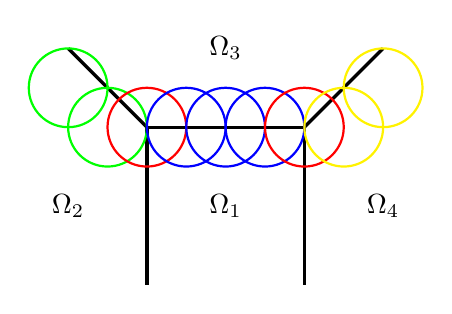
\begin{tikzpicture}
		
		\draw[very thick]  (1,-1) -- (2, -2 );
		\draw[very thick]  (4,-2) --(5,-1);
		%\draw[very thick]  (1,-5) --(2,-4);
		%\draw[very thick] (4,-4)--(5, -5);
		
		\draw[very thick](2,-2)--(4,-2);
		\draw[very thick] (4,-2)--(4,-4);
		%\draw[very thick] (4, -4)--(2, -4);
		\draw[very thick] (2, -4) -- (2, -2);
		

		\draw[green,thick] (1,-1.5) circle (0.5cm);	
		\draw[green,thick] (1.5,-2) circle (0.5cm);	
		\draw[red,thick] (2,-2) circle (0.5cm);	
		\draw[blue,thick] (2.5,-2) circle (0.5cm);	
		\draw[blue,thick] (3,-2) circle (0.5cm);	
		\draw[blue,thick] (3.5,-2) circle (0.5cm);	
		\draw[red,thick] (4,-2) circle (0.5cm);	
		\draw[yellow,thick] (4.5,-2) circle (0.5cm);	
		\draw[yellow,thick] (5,-1.5) circle (0.5cm);	
		
		\node at (3,-3) {$\Omega_{ 1 }$};
		\node at (1,-3) {$\Omega_{2}$};
		\node at (3,-1) {$\Omega_{3}$};
		\node at (5,-3) {$\Omega_{4}$};
	\end{tikzpicture}
	\caption{Localization of multiphase mean curvature flow. For the green 
	balls, we choose the majority phase (2,3), for the blue ones (1,3) and for 
	the yellow balls (3,4). The red balls however give us an error.}
	
	\label{figure_localization_of_mmcf}
\end{figure}

To formulate this rigorously let $ r > 0 $ and define the covering $ \mathcal{ 
B }_{ r 
} $ of the flat torus by
\begin{equation*}
	\mathcal{B}_{ r } \coloneqq
	\left\{
	B_{ r } ( c ) 
	\, \colon \,
	c \in \mathcal{ L }_{ r }
	\right\},
\end{equation*}
where the set of centers $ \mathcal{ L }_{ r } $ is given by $ \mathcal{ L }_{ 
	r } \coloneqq \flattorus \cap (r/\sqrt{ d }) \mathbb{ Z }^{ d } $. Moreover 
	let 
$ \rho_{ B } $ be a smooth cutoff for the ball $ B $ with support in the ball 
with the same center, but double the radius.

Additionally to choosing a majority phase, we can also argue that along the 
chosen majority phase, we have a local flatness. Thus we may approximate the 
outer unit normal up to an arbitrarily small error by a constant unit vector. 
This is captured by the following Lemma found in 
\cite{laux_otto_convergence_of_thresholding_scheme_for_mmcf}. The proof is 
based on De Giorgi's structure theorem for sets of finite perimeter.

\begin{lemma}
	\label{localization_lemma_with_normals}
	For every $ \delta > 0 $ and every partition $ \chi \colon \flattorus \to 
	\{ 0 , 1 \}^{ P } $ such that $ \chi_{ i } \in \bv ( \flattorus ) $ holds 
	for all $ 1 \leq i \leq P $, there exist some $ r_{ 0 } > 0 $ such that for 
	all $ 0 < r < r_{ 0 } $, we find for every ball $ B \in \mathcal{B}_{ r } $ 
	some unit vector $ \nu_{ B } $ such that
	\begin{equation*}
		\sum_{ B \in \mathcal{B}_{ r } }
		\min_{ i \neq j }
		\int
		\rho_{ B }
		\abs{ \nu_{ i } - \nu_{ B } }^{ 2 }
		\abs{ \nabla \chi_{ i } }
		+
		\int
		\rho_{ B }
		\abs{ \nu_{ j } + \nu_{ B } }^{ 2 }
		\abs{ \nabla \chi_{ j } }
		+
		\sum_{ k \notin \{ i , j \} }
		\int 
		\rho_{ B }
		\abs{ \nabla \chi_{ k } }
		\lesssim
		\delta \energy ( \chi ).
	\end{equation*}
\end{lemma}

Note that by \Cref{identities_for_measure_theoretic_boundaries}, integrating  $ 
\abs{ \nabla \chi_{ k } } $ over the sum of all $ k \notin \{ i , j \} $ 
equates to summing over all interfaces which are not the $ (i,j)$-th interface. 
Moreover the second summand is in some sense unnecessary, since the last 
summand provides us with a localization on the $ (i,j)$-th interface, on which 
we have $ \nu_{ i } = - \nu_{ j } $.
However it is convenient to keep it so that we do not have to repeat this 
argument.

\begin{remark}
	\label{localization_estimate_weaker}
	This localization estimate also implies the smallness of
	\begin{equation}
		\label{alternative_localization_equality}
		\sum_{ B \in \mathcal{ B }_{ r } }
		\min_{ i }
		\abs{
			\energy ( \chi; \rho_{ B } )
			-
			\int
			\rho_{ B }
			\abs{ \nabla \psi_{ i } }
		}
		=
		\sum_{ B \in \mathcal{ B }_{ r } }
		\energy ( \chi ; \rho_{ B } )
		-
		\max_{ i }
		\int
		\rho_{ B }
		\abs{ \nabla \psi_{ i } }
	\end{equation}
	in the same sense as in the above \Cref{localization_lemma_with_normals}. 
	Notice that the equality (\ref{alternative_localization_equality}) follows 
	for example from 
	\Cref{supremum_of_abs_nabla_psi_i_is_energy}, which yields that $ \abs{ 
	\nabla 
		\psi_{ i } } \leq \energy ( \chi ; \cdot )$. The smallness follows 
		since by 
	\Cref{rewriting_variation_of_psi_i}, we have for every $ i \neq j $ that
	\begin{align*}
		&
		\energy ( \chi ; \rho_{ B } ) 
		-
		\int
		\rho_{ B }
		\abs{ \nabla \psi_{ i } }
		\\
		={} &
		\sum_{ 1 \leq k < l \leq P }
		\sigma_{ k l }
		\int_{ \Sigma_{ k l } }
		\rho_{ B }
		\dd{ \hm^{ d -1 } }
		-
		\sum_{ 1 \leq k < l \leq P }
		\abs{ \sigma_{ i k } - \sigma_{ i l } }
		\int_{ \Sigma_{ k l } }
		\rho_{ B }
		\dd{ \hm^{ d - 1 } }
		\\
		={} &
		\sum_{ \substack{1 \leq k < l \leq P \\ \{ k, l \} \neq \{ i, j \} } }
		\left(
		\sigma_{ k l } - \abs{ \sigma_{ i k } - \sigma_{ i l } }
		\right)
		\int_{ \Sigma_{ k l } }
		\rho_{ B }
		\dd{ \hm^{ d - 1 } }
		\\
		\lesssim{} &
		\sum_{ k \notin \{ i, j \} }
		\int
		\rho_{ B }
		\abs{ \nabla \chi_{ k } }.
	\end{align*}
	Thus we can estimate the error by the last summand of the error in 
	\Cref{localization_lemma_with_normals}.
\end{remark}
\subsection{Convergence of the curvature term}

\begin{proposition}
	\label{convergence_of_curvature_multiphase}
	In the situation of \Cref{initial_convergence_result_multiphase} and under 
	the energy convergence assumption (\ref{energy_convergence}), we have that 
	the first variations converge in the sense that for almost every time $ 0 
	\leq t \leq T $, we have
	\begin{equation*}
		\lim_{ \varepsilon \to 0 }
		\int
		\inner*{ 
			\varepsilon \Delta u_{ \varepsilon } - \frac{ 1 }{ 
				\varepsilon } \nabla W ( u_{ \varepsilon } ) 
		}
		{ \diff u_{ \varepsilon } \xi } 
		\dd{ x }
		=
		\sum_{ 1 \leq i < j \leq P }
		\sigma_{ i j }
		\int_{ \Sigma_{ i j } }
		\inner*{ \diff \xi }{ \mathrm{Id} - \nu_{ i } \otimes \nu_{ i } }
		\dd{ \hm^{ d - 1} }.
	\end{equation*}
	Additionally we have the estimate
	\begin{equation}
		\label{pointwise_estimate_for_curvature}
		\abs{
		\int
		\inner*{ 
			\varepsilon \Delta u_{ \varepsilon } - \frac{ 1 }{ \varepsilon } 	
			\nabla W ( u_{ \varepsilon } ) }
		{ \diff u_{ \varepsilon } \xi }
		\dd{ x }
		}
		\lesssim
		\norm{ \nabla \xi }_{ \sup }
		\energy_{ \varepsilon } ( u_{ \varepsilon } ).
	\end{equation}
\end{proposition}

\begin{remark}
	\label{difference_twophase_multiphase_curvature}
	We can not proceed exactly as in the twophase case. There the key argument 
	was that from the energy convergence, we could already infer that 
	$ \abs{ \nabla \psi_{ \varepsilon } } ( \flattorus ) $ converges to $ \abs{ 
	\nabla \psi } ( \flattorus ) $, and thus enabled us to apply the Theorem by 
	Reshetnyak. Firstly we do not have one 
	primitive $ \phi $ of $ \sqrt{ 2 W } $ in the multiphase case and more 
	importantly, we can 
	not expect the functions $ 
	\psi_{ \varepsilon ,  i } $ to satisfy 
	\begin{equation}
		\label{energy_convergence_of_psi_i}
		\abs{ \psi_{ \varepsilon ,i } } ( \flattorus ) \to \abs{ \psi_{ i } } ( 
		\flattorus ),
	\end{equation}
	so the original theorem from Reshetnyak will not work here. However we have 
	by the lower semicontinuity of the variation measure under the assumption 
	of energy convergence (\ref{energy_convergence}) that
	\begin{align*}
		\abs{ \nabla \psi_{ i } } ( \flattorus )
		&
		\leq
		\liminf_{ \varepsilon \to 0 }
		\abs{ \nabla \psi_{ \varepsilon , i } } ( \flattorus )
		\\
		& \leq
		\liminf_{ \varepsilon \to 0 }
		\energy_{ \varepsilon } ( u_{ \varepsilon } )
		\\
		& =
		\energy ( u )
		\\
		& =
		\sum_{ 1 \leq j < k \leq P }
		\sigma_{ j k }
		\hm^{ d -1 } ( \Sigma_{ j k } ).
	\end{align*}
	But by \Cref{rewriting_variation_of_psi_i}, we know that
	\begin{equation*}
		\abs{ \nabla \psi_{ i } }
		=
		\sum_{ 1 \leq j < k \leq P }
		\abs{ \sigma_{ i j } - \sigma_{ i k } }
		\hm^{ d - 1 } |_{ \Sigma_{ j k } }.
	\end{equation*}
	Since $ \abs{ \sigma_{ i i } - \sigma_{ i k } } = \sigma_{ i k } $ for all 
	$ k \neq i $,
	this yields that localized on $ \partial_{ \ast } \Omega_{ i } $, we have 
	the necessary convergence $ \abs{ \nabla \psi_{ \varepsilon ,i } } \to 
	\abs{ \nabla \psi_{ i } } $. Thus we will develop a quantitative version of 
	Reshetnyaks theorem and apply it to our setting.
\end{remark}

\begin{proof}[Proof of \Cref{convergence_of_curvature_multiphase}.]
	Using the same calculations as in the two-phase case, we obtain for a given 
	test vector field $ \xi $ that
	\begin{align*}
		& \lim_{ \varepsilon \to 0 }
		\int
		\inner*{
			\varepsilon \Delta u_{ \varepsilon }
			-
			\frac{ 1 }{ \varepsilon } \nabla W ( u_{ \varepsilon } )
		}
		{
			\diff u_{ \varepsilon } \xi
		}
		\dd{ x }
		\\
		={} &
		\lim_{ \varepsilon \to 0 }
		\int
		\varepsilon
		\left(
		\abs{ \nabla u_{ \varepsilon } }^{ 2 }
		\divg \xi 
		-
		\sum_{ i = 1 }^{ N }
		\sum_{ j, k = 1 }^{ d }
		\partial_{ x_{ j } } u_{ \varepsilon }^{ i }
		\partial_{ x_{ j } } \xi^{ k }
		\partial_{ x_{ k } } u_{ \varepsilon }^{ i }
		\right)
		\dd{ x } 
		\eqqcolon 
		\lim_{ \varepsilon \to 0 } I_{ \varepsilon }
	\end{align*}
	Now however, we can not proceed as in the twophase case as explained in 
	\Cref{difference_twophase_multiphase_curvature}. 
	Instead we rewrite
	\begin{equation}
		\label{key_equality_for_ptw_estimate}
		I_{ \varepsilon }
		=
		\int
		\varepsilon
		\inner*{
			\diff \xi 
		}
		{
			\mathrm{Id} - N_{ \varepsilon }^{ \top } N_{ \varepsilon }
		}
		\abs{ \nabla u_{ \varepsilon } }^{ 2 }
		\dd{ x },
	\end{equation}
	where we define $ N_{ \varepsilon } \coloneqq \diff u_{ \varepsilon } / 
	\abs{ \diff u_{ \varepsilon } } $ wherever it is defined, and zero else. 
	By the equipartition of energies 
	(\Cref{equipartition_of_energies_multiphase}) and using that 
	$ \abs{N_{ \varepsilon } } \leq 1 $, we can replace $ \varepsilon \abs{ 
	\nabla u_{ 
	\varepsilon } }^{ 2 } $ by $ \sqrt{ 2 W ( u_{ \varepsilon } ) } \abs{ 
	\nabla u_{ \varepsilon  } } $. 
	
	We can take care of the term involving the divergence again with the 
	equipartition of energies. 
	Thus summarizing our results, it suffices by rescaling to show for all $ 
	A \in \cont^{ \infty } ( \flattorus ; \mathbb{ R }^{ d \times d } ) $ with 
	$ \abs{ A } \leq 1 $ that
	\begin{equation}
		\label{desired_convergence_for_convergence_of_curvature}
		\lim_{ \varepsilon \to 0 }
		\int
		\inner*{ A }{ N_{ \varepsilon }^{ \top } N_{ \varepsilon } }
		\sqrt{ 2 W ( u_{ \varepsilon } ) }
		\abs{ \nabla u_{ \varepsilon } }
		\dd{ x }
		=
		\sum_{ 1 \leq i < j \leq P }
		\sigma_{ i , j }
		\int_{ \Sigma_{ i , j } }
		\inner*{ A }{ \nu_{ i } \otimes \nu_{ i } }
		\dd{ \hm^{ d - 1 } }.
	\end{equation}
	To this end, we will show the following three claims for a partition of 
	unity function $ \eta $.
	\begin{description}[wide=0pt]
		\item[Claim 1:]
		We choose a majority phase by introducing the function $ \phi_{ i } $ 
		on the right hand side of equation 
		(\ref{desired_convergence_for_convergence_of_curvature}). The 
		corresponding error is given by
		\begin{align*}
			& \limsup_{ \varepsilon \to 0 }
			\abs{ 
				\int
				\eta 
				\inner*{ A }{ N_{ \varepsilon }^{ \top } N_{ \varepsilon } }
				\sqrt{ 2 W ( u_{ \varepsilon } ) } \abs{ \nabla u_{ \varepsilon 
				} } 
				\dd{ x }
				-
				\int
				\eta
				\inner*{ A }{ \theta_{ \varepsilon, i } \otimes \theta_{ 
						\varepsilon , i } }
				\abs{ \nabla \psi_{ \varepsilon , i } }
				\dd{ x }
			}
			\\
			\lesssim{} &
			\energy ( u ; \eta ) 
			-
			\int
			\eta
			\abs{ \nabla \psi_{ i } },
		\end{align*}
		where the approximate normal of the $ i$-th phase is defined by $ 
		\theta_{ 
		i }^{ \varepsilon } \coloneqq \nabla \psi_{ i }^{ \varepsilon } / \abs{ 
		\nabla \psi_{ i }^{ \varepsilon } } $ wherever the gradient does not 
		vanish, and zero else.
		
		\item[Claim 2:]
		By a quantitative Reshetnyak type argument, we have
		\begin{equation*}
			\limsup_{ \varepsilon \to 0 }
			\abs{
				\int
				\eta \inner*{ A }{ \theta_{ \varepsilon, i } \otimes \theta_{ 
						\varepsilon,  i } }
				\abs{ \nabla \psi_{ \varepsilon,  i } }
				\dd{ x }
				-
				\int
				\eta \inner*{ A }{ \theta_{ i }  \otimes 
					\theta_{ i } }
				\abs{ \nabla \psi_{ i } }
			}
			\lesssim
			\energy ( u ; \eta ) - \int \eta \abs{ \nabla \psi_{ i } },
		\end{equation*}
		where $ \theta_{ i } \coloneqq \nabla \psi_{ i } / \abs{ \nabla \psi_{ 
				i } } $.
		\item[Claim 3:] 
		We can undo the localization onto the majority phase. The corresponding 
		error is given by
		\begin{equation*}
			\abs{ 
				\int
				\eta
				\inner*{ A }{ \theta_{ i } \otimes \theta_{ i } }
				\abs{ \nabla \psi_{ i } }
				-
				\sum_{ 1 \leq j < k \leq P }
				\sigma_{ j k }
				\int_{ \Sigma_{ j k } }
				\eta 
				\inner*{ A }{ \nu_{ j } \otimes \nu_{ j } }
				\dd{ \hm^{ d - 1 } }
			}
			\leq
			\energy ( u ; \eta ) - \int \eta \abs{ \nabla \psi_{ i } },
		\end{equation*}
		where we remind that $ \nu_{ j } $ is the inner unit normal of $ 
		\Omega_{ j } $.
	\end{description}
	Let us first assume that we have proven those three claims and show how the 
	desired convergence 
	(\ref{desired_convergence_for_convergence_of_curvature}) follows from them. 
	We take a partition of unity $ \eta_{ B } $ of the flat torus with respect 
	to the covering $ \mathcal{ B }_{ r } $ introduced in 
	\Cref{section_localization_estimates}. Then
	\begin{align*}
		& \limsup_{ \varepsilon \to 0 }
		\abs{
			\int
			\inner*{ A }{ N_{ \varepsilon }^{ \top } N_{ \varepsilon } }
			\sqrt{ 2 W ( u_{ \varepsilon } ) }
			\abs{ \nabla u_{ \varepsilon } }
			\dd{ x }
			-
			\sum_{ 1 \leq j < k \leq P }
			\sigma_{ j  k }
			\int_{ \Sigma_{ j k } }
			\inner*{ A }{ \nu_{ j } \otimes \nu_{ j } }
			\dd{ \hm^{ d - 1 } }
		} 
		\\
		={} &
		\abs{ 
			\sum_{ B \in \mathcal{ B }_{ r } }
			\int
			\inner*{ A \eta_{ B } }
			{ N_{ \varepsilon }^{ \top } N_{ \varepsilon } }
			\sqrt{ 2 W ( u_{ \varepsilon } ) } \abs{ \nabla u_{ \varepsilon } }
			\dd{ x }
			-
			\sum_{ 1 \leq j < k \leq P }
			\sigma_{ j k }
			\int_{ \Sigma_{ j k } }
			\inner*{ A \eta_{ B } }
			{ \nu_{ j } \otimes \nu_{ j } }
			\dd{ \hm^{ d - 1 } }
		}
		\\
		\leq{} &
		\sum_{ B \in \mathcal{ B }_{ r } }
		\min_{ 1 \leq i \leq P }
		\abs{ 
			\int
			\inner{ A \eta_{ B } }{ N_{ \varepsilon }^{ \top } N_{ \varepsilon 
			} }
			\sqrt{ 2 W ( u_{ \varepsilon } ) }
			\abs{ \nabla u_{ \varepsilon } }
			\dd{ x }
			-
			\int
			\inner*{ A \eta_{ B } }
			{ \theta_{ \varepsilon , i }\otimes \theta_{ \varepsilon ,i } 
			}
			\abs{ \nabla \psi_{ \varepsilon,  i } }
			\dd{ x }
		}
		\\
		& \quad \quad \quad \;\;\;\!\: +
		\abs{ 
			\int
			\inner*{ A \eta_{ B } }{ \theta_{ \varepsilon ,i } \otimes 
				\theta_{ \varepsilon , i } }
			\abs{ \nabla \psi_{ \varepsilon, i } }
			\dd{ x }
			-
			\int
			\inner*{ A \eta_{ B } }
			{ \theta_{ i } \otimes \theta_{ i } }
			\abs{ \nabla \psi_{ i } }
		}
		\\
		& \quad \quad \quad \;\;\;\!\: +
		\abs{ 
			\int
			\inner*{ A \eta_{ B } }
			{ \theta_{ i } \otimes \theta_{ i } }
			\abs{ \nabla \psi_{ i } }
			-
			\sum_{ 1 \leq j < k \leq P }
			\sigma_{ j k }
			\int_{ \Sigma_{ j k } }
			\inner*{ A \eta_{ B } }
			{ \nu_{ j } \otimes \nu_{ j } }
			\dd{ \hm^{ d - 1 } }
		}
		\\
		\lesssim {} &
		\sum_{ B \in \mathcal{ B }_{ r } }
		\min_{ 1 \leq i \leq P }
		\energy ( u ; \eta_{ B } )
		-
		\int
		\eta_{ B }
		\abs{ \nabla \psi_{ i } },
	\end{align*}
	which vanishes as $ r $ tends to zero by 
	\Cref{localization_estimate_weaker}.
	Thus let us now prove the three claims.
	
	\begin{proof}[Proof of Claim 1.]
		For simplicity, we drop the index $ i $ and for now also $ \varepsilon 
		$.
		First, we replace the matrix $ N $ by the matrix $ \pi N $, where we 
		define the rank-one matrix $ \pi $ by
		\begin{equation*}
			\pi 
			\coloneqq
			\frac{ \nabla \phi }{ \abs{ \nabla \phi } }
			\otimes
			\frac{ \nabla \phi }{ \abs{ \nabla \phi } }
			\in 
			\mathbb{ R }^{ N },
		\end{equation*}
		which is motivated by the chain rule.
		The multiplication with $ \pi $ is an orthogonal projection $ \pi 
		\colon \mathbb{ R }^{ N \times d } \to \mathbb{ R }^{ N \times d } $. 
		Moreover, we can compute that
		\begin{align*}
			( (\pi N)^{ \top } \pi N )_{ i j }
			& =
			\sum_{ k = 1 }^{ N }
			( \pi N )_{ k i }
			( \pi N )_{ k j }
			=
			\sum_{ k = 1 }^{ N }
			\left(
			\sum_{ l = 1 }^{ N }
			\pi_{ k l } N_{ l i }
			\right)
			\left(
			\sum_{ r = 1 }^{ N }
			\pi_{ k r } N_{ r j }
			\right)
			\\
			& =
			\sum_{ l, r = 1 }^{ N }
			N_{ l i } N_{ r j }
			\sum_{ k = 1 }^{ N }
			\pi_{ k l }
			\pi_{ k r }
			=
			\sum_{ l, r = 1 }^{ N }
			N_{ l i }N_{ r j }
			\sum_{ k = 1 }^{ N }
			\frac{ \partial_{ k } \phi  \partial_{ l } \phi \partial_{ 
					k } \phi \partial_{ r } \phi }{ \abs{ \nabla \phi 
				}^{ 4 } }
			\\
			& =
			\sum_{ l, r = 1 }^{ N }
			N_{ l i } \frac{ \partial_{ l } \phi }{ \abs{ \nabla
					\phi } }
			N_{ r j } \frac{ \partial_{ r } \phi }{ \abs{ \nabla 
					\phi } }
			=
			\frac{ \partial_{ i } \psi }{ \abs{ \nabla u } \abs{ \nabla
					\phi } }
			\frac{ \partial_{ j } \psi }{ \abs{ \nabla u } \abs{ \nabla 
					\phi } }
		\end{align*}
		Thus we infer that
		\begin{align}
			\notag
			\inner*{ A }{ ( \pi N_{ \varepsilon })^{ \top } \pi N_{ \varepsilon 
			} }
			& =
			\sum_{ i, j = 1 }^{ d }
			A_{ i j } 
			\frac{ \partial_{ i } \psi_{ \varepsilon } }{ \abs{ \nabla \phi 
				} \abs{ \nabla u_{ \varepsilon } } }
			\frac{ \partial_{ j } \psi_{ \varepsilon } }{ \abs{ \nabla \phi 
				} \abs{ \nabla u_{ \varepsilon } } }
			\\
			\notag
			& =
			\frac{ \abs{ \nabla \psi_{ \varepsilon } }^{ 2 } }{ \abs{ \nabla 
					\phi }^{ 2 } \abs{ \nabla u_{ \varepsilon } }^{ 2 } }
			\inner*{ A }
			{ \frac{ \nabla \psi_{ \varepsilon } }{ \abs{ \nabla \psi_{ 
							\varepsilon } } } \otimes \frac{ \nabla \psi_{ 
							\varepsilon } }{ 
					\abs{ \nabla \psi_{ \varepsilon } } } }
			\\
			\label{rewriting_orthogonal_projection_equation}
			& = 
			\abs{ \pi N_{ \varepsilon } }^{ 2 }
			\inner*{ A }{ \theta_{ \varepsilon } \otimes \theta_{ \varepsilon } 
			},
		\end{align}
		where we used that 
		\begin{equation*}
			\abs{ \pi N_{ \varepsilon } }^{ 2 }
			=
			\frac{ \abs{ \nabla \psi_{ \varepsilon } }^{ 2 } }{ \abs{ \nabla 
					\phi }^{ 2 } \abs{ \nabla u_{ \varepsilon } }^{ 2 } }.
		\end{equation*}
		Moreover we recognize that since multiplication with $ \pi $ is 
		an orthogonal projection, we have the Pythagorean Theorem
		\begin{align*}
			N^{ \top } N 
			& =
			( \pi N + N - \pi N )^{ \top } ( \pi N + N - \pi N )
			\\
			& =
			( \pi N )^{ \top } \pi N 
			+
			( N - \pi N )^{ \top } ( N - \pi N )
			+
			( \pi N )^{ \top } ( N - \pi N )
			+
			( N - \pi N )^{ \top } \pi N 
			\\
			& =
			( \pi N )^{ \top } \pi N
			+
			( N - \pi N )^{ \top } ( N - \pi N ).
		\end{align*}
		In order to prove the claim, we first get an error when replacing $ N_{ 
			\varepsilon }^{ \top } N_{ \varepsilon } $ with 
		$ \theta_{ \varepsilon 
			} 
		\otimes \theta_{ \varepsilon } $ 
		and the second error when replacing 
		$ \sqrt{ 2 W ( u_{ \varepsilon } ) } \abs{ \nabla u_{ \varepsilon } } $ 
		by $ \abs{ \nabla \psi_{ \varepsilon } } $.
		For the first error we can estimate by the Pythagorean Theorem and 
		equation (\ref{rewriting_orthogonal_projection_equation}) that
		\begin{align*}
			& \abs{ 
				\int
				\eta 
				\inner*{ A }{ N_{ \varepsilon }^{ \top } N_{ \varepsilon } }
				\sqrt{ 2 W ( u_{ \varepsilon } ) } \abs{ \nabla u_{ 
						\varepsilon } }
				\dd{ x }
				-
				\int
				\eta
				\inner*{ A }{ \theta_{ \varepsilon } \otimes \theta_{ 
				\varepsilon 
				} }
				\sqrt{ 2 W ( u_{ \varepsilon } ) } \abs{ \nabla u_{ 
						\varepsilon } }
				\dd{ x }
			}
			\\
			\leq{} &
			\abs{ 
				\int
				\eta 
				\inner*{ A }{ N_{ \varepsilon }^{ \top } N_{ \varepsilon } }
				\sqrt{ 2 W ( u_{ \varepsilon } ) } \abs{ \nabla u_{ 
						\varepsilon } } 
				\dd{ x }
				-
				\int 
				\eta
				\inner*{ A }
				{ \pi N_{ \varepsilon }^{ \top } \pi N_{ \varepsilon } }
				\sqrt{ 2 W ( u_{ \varepsilon } ) }
				\abs{ \nabla u_{ \varepsilon } }
				\dd{ x }
			}
			\\
			& + 
			\abs{ 
				\int
				\eta
				\inner*{ A }
				{ \pi N_{ \varepsilon }^{ \top } \pi N_{ \varepsilon } }
				\sqrt{ 2 W ( u_{ \varepsilon } ) } \abs{ \nabla u_{ 
						\varepsilon } }
				\dd{ x }
				-
				\int
				\eta
				\inner*{ A }
				{ \theta_{ \varepsilon } \otimes \theta_{ \varepsilon } }
				\sqrt{ 2 W ( u_{ \varepsilon } ) }
				\abs{ \nabla u_{ \varepsilon } }
				\dd{ x }
			}
			\\
			\leq{} & 
			\int
			\eta
			\abs{ N_{ \varepsilon } - \pi N_{ \varepsilon } }^{ 2 }
			\sqrt{ 2 W ( u_{ \varepsilon} ) } \abs{ \nabla u_{ \varepsilon 
			} }
			\dd{ x }
			+
			\int
			\eta
			\left( 
			1 - \abs{ \pi N_{ \varepsilon } }
			\right)^{ 2 }
			\sqrt{ 2 W ( u_{ \varepsilon } ) } \abs{ \nabla u_{ \varepsilon 
			} }
			\dd{ x }
			\eqqcolon I_{ \varepsilon }.
		\end{align*}
		Using again that multiplication with $ \pi $ is an orthogonal 
		projection, we have
		\begin{align*}
			\abs{
				( \mathrm{Id} - \pi ) N_{ \varepsilon }
			}^{ 2 }
			& =
			\abs{ N_{ \varepsilon } }^{ 2 } 
			-
			\abs{ \pi N_{ \varepsilon } }^{ 2 }
			=
			1 - \abs{ \pi N_{ \varepsilon } }^{ 2 }
			\lesssim
			1 - \abs{ \pi N_{ \varepsilon } }
			=
			1 -
			\abs{ \frac{ \diff \phi }{ \abs{ \nabla \phi } } N_{ \varepsilon } 
			},
		\end{align*}
		where for the last identity, we used that $ \abs{ v^{ \top } B } = 
		\abs{ v \otimes v B } $ for all unit vectors $ v $ and matrices $ B $.
		Therefore we can estimate
		\begin{align*}
			I_{ \varepsilon }
			& \lesssim
			\int
			\eta
			\left(
			1 - \abs{ \frac{ \diff \phi ( u_{ \varepsilon } ) }{ \abs{ \nabla 
			\phi ( u_{ \varepsilon } ) } } N_{ 
					\varepsilon } }
			\right)
			\sqrt{ 2 W ( u_{ \varepsilon } ) }
			\abs{ \nabla u_{ \varepsilon } }
			\dd{ x }
			\\
			& =
			\int
			\eta 
			\left(
			\sqrt{ 2 W ( u_{ \varepsilon } ) }
			\abs{ \nabla u_{ \varepsilon } }
			-
			\abs{ \nabla \psi^{ \varepsilon } }
			\frac{ \sqrt{ 2 W ( u_{ \varepsilon } ) } }{ \abs{ \nabla 
					\phi ( u_{ \varepsilon } ) } }
			\right)
			\dd{ x }
			\\
			& \leq
			\energy_{ \varepsilon } ( u_{ \varepsilon } ; \eta )
			-
			\int
			\eta
			\abs{ \nabla \psi_{ \varepsilon } }
			\dd{ x }.
		\end{align*}
		The last inequality is due to Young's inequality and $ \abs{ \nabla 
			\phi } \leq \sqrt{ 2 W ( u_{ \varepsilon } ) } $.
		By the convergence of energies for almost every time and the lower 
		semicontinuity of the variation measure, we thus have
		\begin{equation*}
			\limsup_{ \varepsilon \to 0 }
			I_{ \varepsilon }
			\lesssim
			\energy ( u ; \eta )
			-
			\int
			\eta
			\abs{ \nabla \psi }.
		\end{equation*}
		The second error is given by
		\begin{align*}
			& \abs{
				\int
				\eta
				\inner*{ A }{ \theta_{ \varepsilon } \otimes \theta_{ 
				\varepsilon 
				} }
				\sqrt{ 2 W ( u_{ \varepsilon } ) }
				\abs{ \nabla u_{ \varepsilon } }
				\dd{ x }
				-
				\int
				\eta
				\inner*{ A }{ \theta_{ \varepsilon } \otimes \theta_{ 
				\varepsilon 
				} }
				\abs{ \nabla \psi_{ \varepsilon } }
				\dd{ x }
			}
			\\
			={} &
			\abs{
				\int
				\eta
				\inner*{ A }{ \theta_{ \varepsilon } \otimes \theta_{ 
				\varepsilon 
				} }
				\left(
				\sqrt{ 2 W ( u_{ \varepsilon } ) } \abs{ \nabla u_{ 
						\varepsilon } } 
				-
				\abs{ \nabla \psi_{ \varepsilon } }
				\right)
				\dd{ x }
			}
			\\
			\leq {} &
			\int
			\eta
			\left(
			\sqrt{ 2 W ( u_{ \varepsilon } ) }
			\abs{ \nabla u_{ \varepsilon } }
			-
			\abs{ \nabla \psi_{ \varepsilon } }
			\right)
			\dd{ x }
			\\
			\leq{} &
			\energy_{ \varepsilon } ( u_{ \varepsilon } ; \eta )
			-
			\int
			\eta 
			\abs{ \nabla \psi_{ \varepsilon } }
			\dd{ x },
		\end{align*}
		which in the limes superior can be controlled by the desired term as 
		above, finishing the proof for the first claim.
	\end{proof}
	
	\begin{proof}[Proof of Claim 2.]
		The strategy here is to first pass to the space of measures in order to 
		obtain some limit, and then sandwich the limit between the measure $ 
		\abs{ \nabla \psi_{ i } } $ and the energy measure $ \energy ( u ; 
		\cdot ) $.
		Thus consider the sequence $ ( \mu_{ \varepsilon } )_{ \varepsilon } $ 
		of 
		Radon measures on $ \flattorus \times \mathbb{ S }^{ d - 1 } $ defined 
		by 
		\begin{equation*}
			\mu_{ \varepsilon }
			\coloneqq
			\abs{ \nabla \psi_{ \varepsilon } } \dd{ x }
			\otimes
			\left( \delta_{ u_{ \varepsilon } ( x ) } \right)_{ x \in 
			\flattorus }
		\end{equation*}
		which acts on continuous functions $ \varphi $ through
		\begin{equation*}
			\int_{ \flattorus \times \mathbb{ S }^{ d - 1 } }
			\varphi ( x , \nu )
			\dd{ \mu_{ \varepsilon } ( x , \nu ) }
			=
			\int_{ \flattorus }
			\varphi \left( x , \nu_{ \varepsilon } ( x ) \right) 
			\abs{ \nabla \psi_{ \varepsilon } }
			\dd{ x }.
		\end{equation*}
		By Young's inequality and the boundedness of energies, $ \mu_{ 
			\varepsilon } $ is a bounded sequence of Radon measures, thus we 
			find a 
		Radon measure $ \tilde{ \mu } $ on $ \flattorus \times \mathbb{ S }^{ d 
			- 1 } $ and some non-relabelled subsequence such that $ \mu_{ 
			\varepsilon } \rightharpoonup^{ \ast } \tilde{ \mu } $ as Radon 
		measures on $ \flattorus \times \mathbb{ S }^{ d - 1 } $.
		By 
		\cite[Thm.~2.28]{ambrosio_fusco_pallara_functions_of_bv_and_free_discontinuity_problems}
		we can disintegrate the measure $ \tilde{ \mu } $, which means that we 
		find probability measures $ ( p_{ x } )_{ x \in \flattorus } $ and a 
		Radon measure $ \mu $ on $ \flattorus $ such that $ x \mapsto p_{ x } $ 
		is $ \mu $-measurable and we have the identity 
		\begin{equation*}
			\int_{ \flattorus \times \mathbb{ S }^{ d - 1 } }
			f ( x , \tilde{ \nu } )
			\dd{ \tilde{ \mu } ( x, \tilde{ \nu } ) }
			=
			\int_{ \flattorus }
			\int_{ \mathbb{ S }^{ d - 1 } }
			f ( x , \tilde{ \nu } )
			\dd{ p_{ x } ( \tilde{ \nu } ) }
			\dd{ \mu ( x ) }
		\end{equation*}
		for all $ f \in \lp^{ 1 } ( \flattorus \times \mathbb{ S }^{ d -1 } , 
		\tilde{ \mu } ) $.
		Thus we have
		\begin{equation*}
			\lim_{ \varepsilon \to 0 }
			\int
			\varphi ( x , \nu_{ \varepsilon } ) 
			\abs{ \nabla \psi^{ \varepsilon } }
			\dd{ x }
			=
			\int_{ \flattorus }
			\int_{ \mathbb{ S }^{ d - 1 } }
			\varphi ( x, \tilde{ \nu } )
			\dd{ p_{ x } ( \tilde{ \nu } ) }
			\dd{ \mu ( x ) }
		\end{equation*} 
		for all continuous $ \varphi $ and plugging in $ \varphi ( x , \tilde{ 
			\nu } ) \coloneqq \inner*{ A ( x ) }{ \tilde{ \nu } \otimes \tilde{ 
			\nu 
		} } $ thus yields
		\begin{equation*}
			\lim_{ \varepsilon \to 0}
			\int
			\eta
			\inner*{ A }{ \nu_{ \varepsilon } \otimes \nu_{ \varepsilon 
			} }
			\abs{ \nabla \psi_{ \varepsilon } }
			\dd{ x }
			=
			\int
			\eta
			\inner*{ A ( x ) }
			{
				\int
				\tilde{ \nu } \otimes \tilde{ \nu }
				\dd{ p_{ x } ( \tilde{ \nu } ) }
			}
			\dd{ \mu ( x ) }.
		\end{equation*}
		We now would like to prove that up to an error bounded by $ \energy ( u 
		; \eta ) - \int \eta \abs{ \nabla \psi } $, the right-hand side is 
		equal to $ \int \inner*{ A }{ \theta \otimes \theta } \abs{ \nabla \psi 
		} $.
		
		On the one hand, we have by the lower semicontinuity of the variation 
		measure that
		\begin{equation}
			\label{mu_doominates_variation_of_psi}
			\int
			\eta
			\abs{ \nabla \psi }
			\leq
			\liminf_{ \varepsilon \to 0 }
			\int
			\eta
			\abs{ \nabla \psi_{ \varepsilon } }
			\dd{ x }
			=
			\int
			\eta ( x )
			\int
			1
			\dd{ p_{ x } ( \tilde{ \nu } ) }
			\dd{ \mu ( x ) }
			=
			\int
			\eta ( x ) 
			\dd{ \mu ( x ) },
		\end{equation}
		or in other words, we have $ \abs{ \nabla \psi } \leq \mu $.
		
		On the other hand we have by the convergence of the energies and 
		Young's inequality that we 
		may estimate $ \mu $ via 
		\begin{equation}
			\label{mu_is_dominated_by_energy}
			\int
			\eta
			\dd{ \mu }
			=
			\lim_{ \varepsilon \to 0 }
			\int
			\eta
			\abs{ \nabla \psi_{ \varepsilon } }
			\dd{ x }
			=
			\liminf_{ \varepsilon \to 0 }
			\energy_{ \varepsilon } ( u_{ \varepsilon } ; \eta )
			=
			\energy ( u ; \eta ).
		\end{equation}
		Using that
		\begin{equation*} 
			\abs{ \tilde{ \nu } \otimes \tilde{ \nu } - \theta \otimes \theta } 
			= 
			\abs{ 
				\tilde{ \nu } \otimes ( \tilde{ \nu } - \theta ) 
				+
				( \tilde{ \nu } - \theta ) \otimes \theta
			}
			\leq
			2 \abs{ \tilde{ \nu } - \theta }
		\end{equation*}
		and inequality (\ref{mu_doominates_variation_of_psi}), we can therefore 
		estimate
		\begin{align*}
			&
			\abs{ 
				\int
				\int_{ \mathbb{ S }^{ d - 1 } }
				\eta
				\inner*{ A }{ \tilde{ \nu } \otimes \tilde{ \nu } }
				\dd{ p_{ x } ( \tilde{ \nu } ) }
				\dd{ \mu }
				-
				\int
				\eta
				\inner*{ A }{ \theta \otimes \theta }
				\abs{ \nabla \psi }
			}
			\\
			\leq{} &
			\abs{ 
				\int
				\eta 
				\inner*{ A }
				{ 
					\int_{ \mathbb{ S }^{ d - 1 } }
					\tilde{ \nu } \otimes \tilde{ \nu }
					\dd{ p_{ x } ( \tilde{ \nu } ) }
				}
				( \dd{ \mu } - \abs{ \nabla \psi } )
			}
			+
			\abs{
				\int
				\eta
				\inner*{ A }{
					\int_{ \mathbb{ S }^{ d - 1 } }
					\tilde{ \nu } \otimes \tilde{ \nu }
					-
					\theta \otimes \theta
					\dd{ p_{ x } ( \tilde{ \nu } ) }
				}
				\abs{ \nabla \psi }
			}
			\\
			\leq {} &
			\int
			\eta
			\left( \dd{ \mu } - \abs{ \nabla \psi } \right)
			+
			2
			\int
			\eta
			\int_{ \mathbb{ S }^{ d - 1 } }
			\abs{ \tilde{ \nu } - \theta } 
			\dd{ p_{ x } ( \tilde{ \nu } ) }
			\abs{ \nabla \psi }.
		\end{align*}
		The first summand can by inequality (\ref{mu_is_dominated_by_energy}) 
		be estimated by 
		$ \energy ( u ; \eta ) - \int \eta \abs{ \nabla \psi } $.
		For the second summand, we use a duality argument:
		Given a smooth vector field $ \xi $, we have by the weak convergence of 
		$ 
		\nabla \psi_{ \varepsilon } $ to $ \nabla \psi $ that
		\begin{equation*}
			\int
			\inner*{ \xi }{ \theta }
			\abs{ \nabla \psi }
			=
			\lim_{ \varepsilon \to 0 }
			\int
			\inner*{ \xi }{ \theta_{ \varepsilon } }
			\abs{ \nabla \psi_{ \varepsilon } }
			\dd{ x }
			=
			\int
			\inner*{ \xi }{
				\int 
				\tilde{ \nu } 
				\dd{ p_{ x } ( \tilde{ \nu } ) } 
			}
			\dd{ \mu },
		\end{equation*}
		from which we deduce that
		\begin{align*}
			\int
			\inner*{ \xi }{
				\int
				\theta - \tilde{ \nu }
				\dd{ p_{ x } ( \tilde{ \nu } ) }
			}
			\abs{ \nabla \psi }
			& =
			\int
			\inner*{ \xi }{
				\int
				\tilde{ \nu }
				\dd{ p_{ x } ( \tilde{ \nu } ) }
			}
			\left(
			\dd{ \mu } - \abs{ \nabla \psi }
			\right)
			\\
			& \leq
			\int
			\abs{ \xi }
			\left(
			\dd{ \mu } - \abs{ \nabla \psi }
			\right)
			\\
			& \leq
			\energy ( u ; \abs{ \xi } )
			-
			\int
			\abs{ \xi }
			\abs{ \nabla \psi },
		\end{align*}
		which finishes the proof.
	\end{proof}
	
	\begin{proof}[Proof of Claim 3.]
		First we notice that since $ \psi_{ i } = \sum_{ j } \sigma_{ i , j } 
		\mathds{ 1 }_{ \Omega_{ j } } $, we have $ \theta_{ i } = \pm \nu_{ j } 
		$ on $ \Sigma_{ j , k } $ $ \abs{ \nabla \psi_{ i } }$ almost 
		everywhere.
		Additionally using the representation of $ \abs{ \nabla \psi_{ i } } $ 
		given in 
		\Cref{rewriting_variation_of_psi_i}, we thus have
		\begin{align*}
			&
			\abs{
				\int
				\eta 
				\inner*{ A }
				{ \theta_{ i } \otimes \theta_{ i } }
				\abs{ \nabla \psi_{ i } }
				-
				\sum_{ 1 \leq j < k \leq P }
				\sigma_{ j k }
				\int_{ \Sigma_{ j k } }
				\eta
				\inner*{ A }{ \nu_{ j } \otimes \nu_{ j } }
				\dd{ \hm^{ d - 1 } }
			}
			\\
			={} &
			\abs{ 
				\sum_{ 1 \leq j < k \leq P }
				\left( 
				\abs{ \sigma_{ i j } - \sigma_{ i k } }
				-
				\sigma_{ j k }
				\right)
				\int_{ \Sigma_{ j k  } }
				\eta
				\inner*{ A }{ \nu_{ j } \otimes \nu_{ j } }
				\dd{ \hm^{ d - 1 } }
			}
			\\
			\leq{} &
			\sum_{ 1 \leq j < k \leq P }
			\int_{ \Sigma_{ j k } }
			\eta
			\left(
			\sigma_{ j  k } - \abs{ \sigma_{ i j } - \sigma_{ i 
					k } }
			\right)
			\dd{ \hm^{ d - 1 } }
			\\
			={} &
			\energy ( u ; \eta )
			-
			\int
			\eta
			\abs{ \nabla \psi_{ i } },
		\end{align*}
		where for the inequality, we used that by the triangle inequality for 
		the surface tensions, we have
		$ \abs{ \sigma_{ i j } - \sigma_{ i k } } \leq \sigma_{ j k } $.
	\end{proof}
	This finishes the proofs for the three claims. Lastly we notice that we 
	obtain the pointwise in time bound (\ref{pointwise_estimate_for_curvature}) 
	from the rewritten term (\ref{key_equality_for_ptw_estimate}).
\end{proof}

We want to point out that Claim 3 and the corresponding proof do not appear in 
\cite{convergence_of_allen_cahn_equation_to_multiphase_mean_curvature_flow}, 
but are necessary in order to finish the proof.

\subsection{Convergence of the velocity term}

As in the previous proof for the convergence of the curvature term we want to 
localize and argue as in the twophase case. Moreover we remember from the 
twophase case that we had to freeze the unit normal. However we now have the 
important difference that $ \nabla u_{ \varepsilon } $ describes both the 
change in physical space (domain) and the state space (codomain). Since the 
supposed limit $ \nu_{ i } $ only describes the change in physical space, we 
should only freeze the normal in this direction. We thus come up with the 
following definition.

\begin{comment}Using the equipartition of 
energies (\Cref{equipartition_of_energies_multiphase}) which tells us that $ 
\varepsilon / 2 \abs{ \nabla u_{ \varepsilon } }^{ 2 } $ roughly equals $ 1 / 
\varepsilon W ( u_{ \varepsilon } ) $, we come up with the following definition 
which is similar to the tilt-excess defined in the twophase case.
\end{comment}

\begin{definition}
	Let $ u _{ \varepsilon } $ and $ \chi $ be as in 
	\Cref{initial_convergence_result_multiphase}.
	Let $ \nu^{ \ast } \in \mathbb{ S }^{ d - 1 } $ and $ \eta \in \cont^{ 
		\infty } \left( [ 0 , T ] \times \flattorus ; [ 0 , 1 ] \right) $. For 
		$ 
	\varepsilon > 0 $  the 
	approximative localized tilt-excess of the $ i$-th phase is given by
	\begin{equation*}
		\tilt_excess_{ i }^{ \varepsilon } ( \nu^{ \ast } ; \eta )
		\coloneqq
		\int_{ 0 }^{ T }
		\int
		\eta
		\frac{ 1 }{ \varepsilon }
		\abs{ 
			\varepsilon \diff u_{ \varepsilon } 
			+
			\nabla \phi_{ i } ( u_{ \varepsilon } ) 
			\otimes
			\nu^{ \ast }
		}^{ 2 }
		\dd{ x }
		\dd{ t }.
	\end{equation*}
	In the limit $ \varepsilon = 0 $,
	we define the tilt-excess for $ 1 \leq i, j \leq P $ , $ i \neq j $ to be
	\begin{equation*}
		\tilt_excess_{ i j } ( \nu^{ \ast } ; \eta  ) 
		\coloneqq
		\int_{ 0 }^{ T }
		\int
		\eta
		\abs{ \nu_{ i } - \nu^{ \ast } }^{ 2 }
		\abs{ \nabla \chi_{ i } }
		\dd{ t }
		+
		\int_{ 0 }^{ T }
		\int
		\eta
		\abs{ \nu_{ j } + \nu^{ \ast } }^{ 2 }
		\abs{ \nabla \chi_{ j } }
		\dd{ t }
		+
		\sum_{ k \in \{ i , j \} }
		\int_{ 0 }^{ T }
		\int
		\eta 
		\abs{ \nabla \chi_{ k } }
		\dd{ t }.
	\end{equation*}
\end{definition}

Notice that we use $ + \nabla \phi_{ i } ( u_{ \varepsilon } ) \otimes \nu^{ 
	\ast } $ in the definition of the approximate tilt excess instead of its 
negative since the normal of $ \chi_{ i } $ points inwards with respect to $ 
\Omega_{ i } $, but $ \nabla \phi_{ i } / \abs{ \nabla \phi_{ i } } $ points 
away from $ \Omega_{ i } $.

Moreover we want to point out that the first two summands of the tilt-excess $ 
\tilt_excess_{ i j } $ measure the local flatness of the boundary, and the 
last summand measure if mostly the $(i,j)$-th phase is present, see also the 
discussion in \Cref{section_localization_estimates}.

As in the twophase case, we first want to argue that when $ \varepsilon $ 
approaches zero, the approximate tilt-excess can be bounded by the tilt-excess 
of the limit.

\begin{lemma}
	\label{approximate_tilt_excess_estimated_in_limit_by_tilt_excess}
	Assume that we are in the situation of 
	\Cref{initial_convergence_result_multiphase} and that the time-integrated 
	energies converge (\ref{energy_convergence}). Then for every $ 1 \leq i , j 
	\leq P $ with $ i \neq j $, every unit vector $ \nu^{ \ast } \in \mathbb{ S 
	}^{ d - 1 } $ and 
	$ \eta \in \cont^{ \infty } \left( [ 0 , T ] \times \flattorus ; [ 0 ,1 ] 
	\right) $, we have
	\begin{equation*}
		\limsup_{ \varepsilon \to 0 }
		\tilt_excess_{ i }^{ \varepsilon } ( \nu^{ \ast } ; \eta  ) 
		\lesssim
		\tilt_excess_{ i j } ( \nu^{ \ast } ; \eta ).
	\end{equation*}
\end{lemma}

\begin{proof}
	By expanding the square, we see that we can rewrite the approximate 
	tilt-excess as
	\begin{align*}
		& \tilt_excess_{ i }^{ \varepsilon } ( \nu^{ \ast } ; \eta ) 
		\\
		={} &
		\int_{ 0 }^{ T }
		\int
		\eta
		\frac{ 1 }{ \varepsilon }
		\left(
		\varepsilon^{ 2 }
		\abs{ \diff u_{ \varepsilon } }^{ 2 }
		+
		2 \varepsilon 
		\inner*{ \diff u_{ \varepsilon } }
		{ \nabla \phi_{ i } ( u_{ \varepsilon } ) \otimes \nu^{ 
				\ast } }
		+
		\abs{ \nabla \phi_{ i } ( u_{ \varepsilon } ) \otimes \nu^{ 
				\ast } }^{ 2 }
		\right)
		\dd{ x }
		\dd{ t }
		\\
		\eqqcolon {} &
		A_{ \varepsilon } + B_{ \varepsilon } + C_{ \varepsilon}.
	\end{align*}
	Using the equipartition of energies 
	(\Cref{equipartition_of_energies_multiphase}), we immediately get that 
	\begin{align*}
		\limsup_{ \varepsilon \to 0 }
		A_{ \varepsilon }
		& =
		\int_{ 0 }^{ T }
		\energy ( u ; \eta )
		\dd{ t }
		\shortintertext{and}
		\limsup_{ \varepsilon \to 0 }
		C_{ \varepsilon }
		& \leq
		\limsup_{ \varepsilon \to 0 }
		\int_{ 0 }^{ T }
		\int
		\eta
		\frac{ 1 }{ \varepsilon }
		\abs{ \nabla \phi_{ i } ( u_{ \varepsilon } ) }^{ 2 }
		\dd{ x }
		\dd{ t }
		\\
		& \leq
		\limsup_{ \varepsilon \to 0 }
		\int_{ 0 }^{ T }
		\int
		\eta
		\frac{ 1 }{ \varepsilon }
		2 W ( u_{ \varepsilon } ) 
		\dd{ x }
		\dd{ t }
		\\
		& =
		\int_{ 0 }^{ T }
		\energy ( u ; \eta )
		\dd{ t }.
	\end{align*}
	For the remaining summand, we note that
	\begin{equation*}
		\limsup_{ \varepsilon \to 0 }
		B_{ \varepsilon }
		=
		\limsup_{ \varepsilon \to 0 }
		\int_{ 0 }^{ T }
		\int
		2 \eta
		\inner*{ \nu^{ \ast } }{ \nabla \psi_{ \varepsilon , i } }
		\dd{ x }
		\dd{ t }
		=
		\int_{ 0 }^{ T }
		\int
		2 \eta
		\inner*{ \nu^{ \ast } }{ \nabla \psi_{ i } }
		\dd{ t }.
	\end{equation*}
	Summarizing these estimates, we have
	\begin{equation*}
		\limsup_{ \varepsilon \to 0 }
		\tilt_excess_{ i }^{ \varepsilon }
		( \nu^{ \ast } ; \eta , u_{ \varepsilon } )
		\leq
		2 \int_{ 0 }^{ T }
		\energy ( u ; \eta )
		\dd{ t }
		+
		2 \int_{ 0 }^{ T }
		\int
		\eta
		\inner*{ \nu^{ \ast } }{ \nabla \psi_{ i } }
		\dd{ t }.
	\end{equation*}
	By focusing on the $ ( i, j )$-th interface, we estimate the energy term by
	\begin{equation*}
		\int_{ 0 }^{ T }
		\energy ( u ; \eta )
		\dd{ t }
		\leq
		\int_{ 0 }^{ T }
		\sigma_{ i j }
		\int
		\eta
		\abs{ \nabla \chi_{ j } }
		\dd{ t }
		+
		C \sum_{ k \notin \{ i , j \} }
		\int_{ 0 }^{ T }
		\int
		\eta
		\abs{ \nabla \chi_{ k } }
		\dd{ t }
	\end{equation*}
	and the other term via
	\begin{align*}
		\int_{ 0 }^{ T }
		\inner*{ \nu^{ \ast } }
		{
			\int
			\eta
			\nabla \psi_{ i }
		}
		\dd{ t }
		& =
		\sum_{ 1 \leq k \leq P }
		\sigma_{ i k }
		\int_{ 0 }^{ T }
		\inner*{ \nu^{ \ast } }
		{
			\int
			\eta 
			\nabla \chi_{ k }
		}
		\dd{ t }
		\\
		& \leq
		\int_{ 0 }^{ T }
		\sigma_{ i j }
		\int
		\eta
		\inner*{ \nu^{ \ast } }{ \nu }
		\abs{ \nabla \chi_{ j } }
		+
		C \sum_{ k \notin \{ i , j \} }
		\int_{ 0 }^{ T }
		\int
		\eta
		\abs{ \nabla \chi_{ k } }
		\dd{ t },
	\end{align*}
	which yields that
	\begin{equation*}
		\limsup_{ \varepsilon \to 0 }
		\tilt_excess_{ i }^{ \varepsilon } ( \nu^{ \ast } ; \eta )
		\leq
		2 \sigma_{ i j } \int_{ 0 }^{ T }
		\int
		\eta
		\left( 1 + \inner*{ \nu^{ \ast } }{ \nu_{ j } } \right)
		\abs{ \nabla \chi_{ j } }
		\dd{ t }
		+
		C \sum_{ k \notin \{ i , j \} }
		\int_{ 0 }^{ T }
		\int
		\eta 
		\abs{ \nabla \chi_{ k } }
		\dd{ t }.
	\end{equation*}
	Since $ 1 + \inner*{ \nu^{ \ast } }{ \nu_{ j } } = \frac{ 1 }{ 2 } \abs{ 
		\nu^{ \ast } + \nu_{ j } }^{ 2 } $, this finishes the proof.
\end{proof}

Note that we have actually proven a seemingly stronger estimate, since the 
summand $ \abs{ \nu_{ i } - \nu^{ \ast } } $ is not included on the right-hand 
side of the last estimate. However it serves to symmetrize the multiphase 
excess.

Using \Cref{approximate_tilt_excess_estimated_in_limit_by_tilt_excess}, we can 
now prove a localized version of the convergence of the velocity term.

\begin{proposition}
	\label{convergence_of_velocity_multiphase}
	In the situation of \Cref{initial_convergence_result_multiphase} and under 
	the assumption that the time-integrated energies converge 
	(\ref{energy_convergence}), there exists a finite Radon measure $ \mu $ on 
	$ [ 0 , T ] \times \flattorus $ such that for every $ 1 \leq i , j \leq P $ 
	with $ i \neq j $, every parameter $ \alpha \in ( 0 , 1 ) $, every unit 
	vector $ \nu^{ \ast } \in \mathbb{ S }^{ d - 1 } $ and every test vector 
	field $ \xi \in \cont_{ \mathrm{c} }^{ \infty } \left( ( 0 , T ) \times 
	\flattorus ; \mathbb{ R }^{ d } \right) $, we have
	\begin{align*}
		& \limsup_{ \varepsilon \to 0 }
		\abs{
			\int_{ 0 }^{ T }
			\int
			\varepsilon
			\inner*{ \partial_{ t } u_{ \varepsilon } }{ \diff u_{ 
					\varepsilon } \eta \xi }
			\dd{ x }
			\dd{ t }
			-
			\sigma_{ i j }
			\int_{ 0 }^{ T }
			\int_{ \Sigma_{ i j } }
			\inner*{ \eta \xi }{ \nu_{ i } } V_{ i }
			\dd{ \hm^{ d - 1 } }
			\dd{ t }
		}
		\\
		\lesssim{} &
		\norm{ \xi }_{ \mathrm{sup} }
		\left(
		\frac{ 1 }{ \alpha } \tilt_excess_{ i j } \left( \nu^{ \ast } ; 
		\eta \right) 
		+ \alpha \mu ( \eta ) 
		\right).
	\end{align*}
	Here $ \eta \in \cont^{ \infty } \left( [ 0 , T ] \times \flattorus ;  
	[ 0 , 1 ]
	\right) $ is some partition of unity function.
\end{proposition}

\begin{proof}
	On a technical note, we first pass to a non-relabelled subsequence such 
	that the limes superior becomes the regular limit.
	As in the twophase case, we first choose a majority phase and then freeze 
	the approximate normal $ \varepsilon \nabla u_{ \varepsilon } $ by 
	replacing it with $ - \nabla \phi_{ i } ( u_{ \varepsilon } ) \otimes \nu^{ 
	\ast } $. The error we can be estimated by Young's inequality through
	\begin{align}
		\notag
		& \abs{
			\int_{ 0 }^{ T }
			\int
			\varepsilon
			\inner*{ \partial_{  t } u_{ 
					\varepsilon } }{ \diff u_{ \varepsilon } \eta \xi }
			\dd{ x }
			\dd{ t }
			+
			\int_{ 0 }^{ T }
			\int
			\inner*{ \partial_{ t } u_{ \varepsilon } }{ \nabla \phi_{ 
					i } ( u_{ \varepsilon } ) \otimes 
				\nu^{ \ast } \eta\xi }
			\dd{ x }
			\dd{ t }
		}
		\\
		\notag
		={} &
		\abs{
			\int_{ 0 }^{ T }
			\int
			\inner*
			{ 
				\sqrt{ \varepsilon } \partial_{ t } u_{ \varepsilon } }{ 
				\left(
				\sqrt{ \varepsilon } \diff u_{ \varepsilon }
				+
				\frac{ 1 }{ \sqrt{ \varepsilon } }
				\nabla \phi_{ i } \otimes \nu^{ \ast } 
				\right)
				\eta \xi 
			}
			\dd{ x }
			\dd{ t }
		}
		\\
		\label{first_error_for_velocity}
		\leq{} &
		\frac{ 1 }{ 2 }
		\norm{ \xi }_{ \mathrm{sup} }
		\left(
		\alpha 
		\int_{ 0 }^{ T }
		\int
		\eta \varepsilon 
		\abs{ \partial_{ t } u_{ \varepsilon } }^{ 2 }
		\dd{ x }
		\dd{ t }
		+
		\frac{ 1 }{ \alpha }
		\tilt_excess_{ i }^{ \varepsilon } \left( \nu^{ \ast } ; \eta \right)
		\right).
	\end{align}
	We thus have arrived at the term
	\begin{equation*}
		- \int_{ 0 }^{ T }
		\int
		\inner*{ \partial_{ t } u_{ \varepsilon } }{ \nabla \phi_{ i } 
			( u_{ \varepsilon } ) \otimes \nu^{ 
				\ast } \eta \xi }
		\dd{ x }
		\dd{ t }
		= 
		- \int_{ 0 }^{ T }
		\int
		\partial_{ t } \psi_{ \varepsilon , i }
		\inner*{ \eta \xi }{ \nu^{ \ast } }
		\dd{ x }
		\dd{ t },
	\end{equation*} 
	which by the weak convergence of $ \partial_{ t } \psi_{ \varepsilon,  i } 
	$ to $ \partial_{ t } \psi_{ i } $ converges to
	\begin{equation*}
		- \sum_{ 1 \leq j \leq P }
		\sigma_{ i j }
		\int_{ 0 }^{ T }
		\int
		\inner*{ \eta \xi }{ \nu^{ \ast } }
		V_{ j }
		\abs{ \nabla \chi_{ j } }
		\dd{ t }.
	\end{equation*}
	Thus
	\begin{align*}
		& \limsup_{ \varepsilon \to 0 }
		\abs{
			- \int_{ 0 }^{ T }
			\int
			\inner*{ \partial_{ t } u_{ 
					\varepsilon } }{ \nabla \phi_{ i } ( u_{ 
					\varepsilon } ) 
				\otimes \nu^{ \ast } \eta \xi }
			\dd{ x }
			\dd{ t }
			-
			\sigma_{ i j }
			\int_{ 0 }^{ T }
			\int_{ \Sigma_{ i j } }
			\inner*{ \eta \xi }{ \nu_{ i } }
			V_{ i } 	
			\dd{ \hm^{ d - 1 } }
			\dd{ t }
		}
		\\
		={} &
		\abs{
			\sum_{ 1 \leq k \leq P }
			\sigma_{ i k }
			\int_{ 0 }^{ T }
			\int
			\inner*{ \eta \xi }{ \nu^{ \ast } }
			V_{ k }
			\abs{ \nabla \chi_{ k } }
			\dd{ t }
			+
			\sigma_{ i j }
			\int_{ 0 }^{ T }
			\int_{ \Sigma_{ i j } }
			\inner*{ \eta \xi }{ \nu_{ i } }
			V_{ i }
			\dd{ \hm^{ d - 1 } }
			\dd{ t }
		}
		\\
		\lesssim{} &
		\norm{ \xi }_{ \mathrm{sup} }
		\sum_{ k \notin \{ i , j \} }
		\int_{ 0 }^{ T }
		\int
		\eta
		\abs{ V_{ k } }
		\abs{ \nabla \chi_{ k } }
		\dd{ t }
		+
		\abs{
			\int_{ 0 }^{ T }
			\int_{ \Sigma_{ i j } }
			\left(
			-\inner*{ \eta \xi }{ \nu^{ \ast } }
			+
			\inner*{ \eta \xi }{ \nu_{ i } }
			\right)
			V_{ i }
			\dd{ \hm^{ d -1 } }
			\dd{ t }
		}.
	\end{align*}
	By applying Young's inequality twice and using again that on $ \Sigma_{ i j 
	} 
	$, we have $ V_{ 
		i } = - V_{ j } $, we furthermore estimate this term by
	\begin{align*}
		& \norm{ \xi }_{ \mathrm{sup} }
		\left(
		\sum_{ k \notin \{ i , j \} }
		\alpha 
		\int_{ 0 }^{ T }
		\int
		\eta
		\abs{ V_{ k } }^{ 2 }
		\abs{ \nabla \chi_{ k } }
		\dd{ t }
		+
		\frac{ 1 }{ \alpha }
		\int_{ 0 }^{ T }
		\int
		\eta
		\abs{ \nabla \chi_{ k } }
		\dd{ t }
		+
		\int_{ 0 }^{ T }
		\int_{ \Sigma_{ i j } }
		\eta
		\abs{ V_{ i } }
		\abs{ \nu^{ \ast } - \nu_{ i } }
		\dd{ \hm^{ d - 1 } }
		\dd{ t }
		\right)
		\\
		\leq{} &
		\norm{ \xi }_{\mathrm{sup} }
		\left(
		\alpha
		\sum_{ 1 \leq k \leq P }
		\int_{ 0 }^{ T }
		\int
		\eta
		\abs{ V_{ k } }^{ 2 }
		\abs{ \nabla \chi_{ k } }
		\dd{ t}
		+
		\frac{ 1 }{ \alpha }
		\tilt_excess_{ i j } ( \nu^{ \ast } ; \eta )
		\right).
	\end{align*}
	By looking again at the first error we made in inequality 
	(\ref{first_error_for_velocity}), we therefore define the measure $ \mu $ 
	through
	\begin{equation*}
		\mu
		\coloneqq
		\sum_{ 1 \leq k \leq P }
		\abs{ V_{ k } }^{ 2 }
		\abs{ \nabla \chi_{ k } }
		\dd{ t }
		+
		\mu_{ 2 },
	\end{equation*}
	where $ \mu_{ 2 } $ is the weak-star limit of some non-relabelled 
	subsequence of the Radon measures $ \varepsilon \abs{ \partial_{ t } u_{ 
			\varepsilon } }^{ 2 } \dd{ x } \dd{ t } $, which stay bounded due 
			to the 
	energy dissipation inequality (\ref{energy_dissipation_sharp}).
	This defines a finite Radon measure on $ [ 0 , T ] \times \flattorus $ by 
	the square-integrability of the velocities observed in 
	\Cref{existence_and_square_integrability_of_velocities_multiphase} and 
	thus, the proof is complete.
\end{proof}

We are now in the position to prove the main result 
\Cref{convergence_to_multiphase_mcf}. This still requires some effort and the 
argument for the localization in time is missing in 
\cite{convergence_of_allen_cahn_equation_to_multiphase_mean_curvature_flow}.

\begin{proof}[Proof of \Cref{convergence_to_multiphase_mcf}.]
	Let us first collect all previous results.
	\Cref{initial_convergence_result_multiphase} guarantees that a limit $ \chi 
	$  as described in \Cref{convergence_to_multiphase_mcf} exists.
	After that \Cref{continuity_in_l2_and_initial_data_multiphase} ensures that 
	$ \chi $ is continuous in time with respect to the $ \lp^{ 2 } $-norm and 
	therefore assumes the initial data. The existence of square-integrable 
	normal velocities is proven in 
	\Cref{existence_and_square_integrability_of_velocities_multiphase}.
	For the 
	distributional equation, the convergence of the curvature term has been 
	proven in
	\Cref{convergence_of_curvature_multiphase}. 
	Thus we still need the full 
	convergence of the velocity term, and the bulk of the work has already been 
	done in \Cref{convergence_of_velocity_multiphase}.
	We see that the only thing left to show is the full convergence 
	of the velocity term, which states that
	\begin{equation*}
		\lim_{ \varepsilon \to 0 }
		\int_{ 0 }^{ T }
		\int
		\varepsilon
		\inner*{ \partial_{ t } u_{ 
				\varepsilon } }{ \diff u_{ \varepsilon } \xi }
		\dd{ x }
		\dd{ t }
		=
		\sum_{ 1 \leq i < j \leq P }
		\sigma_{ i j }
		\int_{ 0 }^{ T }
		\int_{ \Sigma_{ i j } }
		\inner*{ \xi }{ \nu_{ i } }
		V_{ i }
		\dd{ \hm^{ d - 1 } }
		\dd{ t }.
	\end{equation*} 
	The key problem we are facing is that the localization estimate 
	\Cref{localization_lemma_with_normals} states that if we can choose the 
	majority phase for a fixed time, then we expect smallness. However we see 
	that the definition of the tilt-excess yields only a time-integrated error. 
	Thus we want to take a partition of unity also in time and control the 
	error.
	
	To this end, let $ 0 = T_{ 0 } < \dotsc < T_{ k } = T $ be a partition of $ 
	[ 0 , T ] $ and for a given $ \delta > 0 $, let $ ( g_{ k } )_{ k = 1 , 
		\dotsc, K } $ be a partition of unity with respect to the intervals 
	$ \left( ( T_{ k - 1 } - \delta , T_{ k } + \delta ) \right) $. As before 
	let $ \eta_{ B } $ be a partition of unity in space with respect to the 
	covering $ \mathcal{ B }_{ r } $. 
	Then for any parameter $ \alpha \in ( 0 , 
	1 ) $, we compute that by \Cref{convergence_of_velocity_multiphase}, we have
	\begin{align*}
		A \coloneqq&
		\limsup_{ \varepsilon \to 0 }
		\abs{
			\int_{ 0 }^{ T }
			\int
			\varepsilon
			\inner*{ \partial_{ t } 
				u_{ \varepsilon } }{ \diff u_{ \varepsilon } \xi }
			\dd{ x }
			\dd{ t }
			-
			\sum_{ 1 \leq i < j \leq P }
			\sigma_{ i j }
			\int_{ 0 }^{ T }
			\int_{ \Sigma_{ i j } }
			\inner*{ \xi }{ \nu_{ i } }
			V_{ i }
			\dd{ \hm^{ d -1 } }
			\dd{ t }
		}
		\\
		\leq{} &
		\sum_{ k = 1 }^{ K }
		\sum_{ B \in \mathcal{ B }_{ r } }
		\limsup_{ \varepsilon \to 0 }
		\Bigg{|}
		\int_{ 0 }^{ T }
		\int
		\varepsilon
		g_{ k } \eta_{ B }
		\inner*{ 
			\partial_{ t } u_{ \varepsilon } }{ \diff 
			u_{ \varepsilon } \xi }
		\dd{ x }
		\dd{ t }
		\\
		& \qquad \qquad \qquad \qquad-
		\sum_{ 1 \leq i < j \leq P }
		\sigma_{ i j }
		\int_{ 0 }^{ T }
		\int_{ \Sigma_{ i j } }
		g_{ k } \eta_{ B }
		\inner*{\xi }{ \nu_{ i } }
		V_{ i }
		\dd{ \hm^{ d - 1 } }
		\dd{ t }					
		\Bigg{|}
		\\
		\lesssim{} &
		\norm{ \xi }_{ \mathrm{sup} }
		\sum_{ k = 1 }^{ K }
		\sum_{ B \in \mathcal{ B }_{ r } }
		\min_{ i \neq j }
		\min_{ \nu^{ \ast } \in \mathbb{ S }^{ d - 1 } }
		\frac{ 1 }{ \alpha }
		\tilt_excess_{ i j } ( \nu^{ \ast } ; g_{ k } \eta_{ 
			B } )
		+
		\alpha \mu ( g_{ k } \eta_{ B } )
	\end{align*}
	Since no derivative falls on $ g_{ k } $, this term converges as $ \delta $ 
	tends to zero to
	\begin{align}
		\label{error_for _convergence_of_velocity}
		\norm{ \xi }_{ \mathrm{sup} }
		\alpha \mu \left( [ 0 , T ] \times \flattorus \right)
		+
		\norm{ \xi }_{ \mathrm{sup} }
		\frac{ 1 }{ \alpha }
		\sum_{ k = 1 }^{ K }
		\sum_{ B \in \mathcal{ B }_{ r } }
		& \min_{ i \neq j }
		\min_{ \nu^{ \ast } \in \mathbb{ S }^{ d - 1 } }
		\int_{ T_{ k - 1 } }^{ T_{ k } }
		\int
		\eta_{ B } 
		\abs{ \nu_{ i } - \nu^{ \ast } }^{ 2 }
		\abs{ \nabla \chi_{ i } }
		\\
		\notag
		+ &
		\int
		\eta_{ B }
		\abs{ \nu_{ j } + \nu^{ \ast } }^{ 2 }
		\abs{ \nabla \chi_{ j } }
		+ 
		\sum_{ k \notin \{ i , j \} }
		\int
		\eta_{ B }
		\abs{ \nabla \chi_{ k } }
		\dd{ t }.
	\end{align}
	Our problem is now that we would like to take the majority phase 
	approximate inner normal dependent on time, which equates to pulling both 
	minima inside the time integral. If our partition $ \chi $ is smooth, then 
	by choosing partitions $ ( T_{ k } )_{ k = 1 , \dotsc, K } $ whose width 
	goes to zero, this would be possible. Since our partition will in general 
	not be smooth, we instead choose a smooth approximation $ \chi^{ n } $ 
	which converges to $ \chi $ with respect to the strict metric as $ n $ 
	tends to infinity. We estimate 
	that for every $ 1 \leq i \leq P $, every unit vector $ \nu^{ \ast } \in 
	\mathbb{ S }^{ d - 1 } $, fixed index $ k $ and ball $ B $, we have that 
	when replacing $ \chi $ with $ \chi^{ n } $ in  a summand of equation 
	(\ref{error_for 
		_convergence_of_velocity}), we get an error of size at most
	\begin{align*}
		& \int_{ T_{ k - 1 } }^{ T_{ k } }
		\abs{ 
			\int
			\eta_{ B }
			\abs{
				\nu_{ i } - \nu^{ \ast }
			}^{ 2 }
			\abs{ \nabla \chi_{ i } }
			-
			\int
			\eta_{ B }
			\abs{ \nu_{ i }^{ n } - \nu^{ \ast } }^{ 2 }
			\abs{ \nabla \chi_{ i }^{ n } }
		}
		\\
		& +
		\abs{
			\int
			\eta_{ B } 
			\abs{ \nu_{ j } + \nu^{ \ast } }^{ 2 }
			\abs{ \nabla \chi_{ j } }
			-
			\int
			\eta_{ B }
			\abs{ \nu_{ j }^{ n } + \nu^{ \ast } }^{ 2 }
			\abs{ \nabla \chi_{ j }^{ n } }
		}
		+
		\sum_{ l \notin \{ i , j \} }
		\abs{
			\int
			\eta_{ B }
			\abs{ \nabla \chi_{ l } }
			-
			\int
			\eta_{ B }
			\abs{ \nabla \chi_{ l }^{ n } }
		}
		\dd{ t }
		\\
		\lesssim{} &
		\sum_{ l = 1 }^{ P }
		\int_{ T_{ k - 1 } }^{ T_{ k } }
		\abs{ 
			\int
			\eta_{ B }
			\abs{ \nabla \chi_{ l } }
			-
			\int
			\eta_{ B }
			\abs{ \nabla \chi_{ l }^{ n } }
		}
		+
		\abs{ 
			\int
			\eta_{ B }
			\nu_{ l }
			\abs{ \nabla \chi_{ l } }
			- 
			\int
			\eta_{ B }
			\nu_{ l }^{ n }
			\abs{ \nabla \chi_{ l }^{ n } }
		}
		\dd{ t }.
	\end{align*}
	Here $ \nu_{ i }^{ n }$ is defined by $ \nabla \chi_{ i }^{ n } / \abs{ 
		\nabla \chi_{ i }^{ n } } $, and for the inequality we used that $ 
		\abs{ 
		\vartheta - \gamma }^{ 2 } = 2( 1 - \inner*{ \vartheta }{ \gamma } ) $ 
		for 
		unit 
	vectors $ \vartheta $ and $ \gamma $. Thus when replacing $ \chi $ by $ 
	\chi^{ 
		n } $ in (\ref{error_for _convergence_of_velocity}), we get an error of 
		size
	at most
	\begin{equation*}
		\frac{ 1 }{ \alpha }
		\sum_{ B \in \mathcal{ B }_{ r } }
		\int_{ 0 }^{ T }
		\sum_{ 1 \leq l \leq P }
		\abs{ 
			\int
			\eta_{ B }
			\abs{ \nabla \chi_{ l } }
			-
			\int
			\eta_{ B }
			\abs{ \nabla \chi_{ l }^{ n } }
		}
		+
		\abs{
			\int
			\eta_{ B }
			\nu_{ l } 
			\abs{ \nabla \chi_{ l } }
			-
			\int
			\eta_{ B }
			\nu_{ l }^{ n }
			\abs{ \nabla \chi_{ l }^{ n } }
		}
		\dd{ t },
	\end{equation*}
	which can be made arbitrarily small independent of the partition of $ [ 0 , 
	T ] $ we have chosen when we let $ n $ tend to infinity.
	Since $ \chi^{ n } $ is smooth, we can now make the width of our partition 
	arbitrarily small and therefore obtain that
	\begin{alignat*}{2}
		A 
		\lesssim{} &
		\norm{ \xi }_{\mathrm{sup}}
		\alpha \mu \left( [ 0 , T ] \times \flattorus \right)
		+
		\delta ( n )
		\\
		& +
		\norm{ \xi }_{ \mathrm{sup}}
		\frac{ 1 }{ \alpha }
		\int_{ 0 }^{ T }
		\sum_{ B \in \mathcal{ B }_{ r } }
		\min_{ i \neq j }
		\min_{ \nu^{ \ast } \in \mathbb{ S }^{ d - 1 } }
		\int
		\rho_{ B }
		\abs{ \nu_{ i }^{ n } - \nu^{ \ast } }^{ 2 }
		\abs{ \nabla \chi_{ i }^{ n } }
		& +
		\int
		\rho_{ B }
		\abs{ \nu_{ j }^{ n } + \nu^{ \ast } }^{ 2 }
		\abs{ \nabla \chi_{ j }^{ n } }
		\\
		& &
		+
		\sum_{ k \notin \{ i , j \} }
		\int
		\rho_{ B }
		\abs{ \nabla \chi_{ k }^{ n } }
		\dd{ t },
	\end{alignat*}
	where $ \delta ( n ) $ is some positive number which tends to zero as n 
	approaches infinity.
	Now letting $ n $ tend to infinity yields by the generalized dominated 
	convergence theorem with majorant 
	$ C \sum_{ i } \int \eta_{ B } \abs{ \nabla \chi_{ i }^{ n } } $ 
	(whose time integral converges due to the strict convergence)
	that
	\begin{alignat*}{2}
		A 
		\lesssim &
		\norm{ \xi }_{ \mathrm{sup} }
		\alpha
		\mu \left(
		[ 0 , T ] \times \flattorus
		\right)
		\\
		& +
		\norm{ \xi }_{ \mathrm{sup} }
		\frac{ 1 }{ \alpha }
		\int_{ 0 }^{ T }
		\sum_{ B \in \mathcal{ B }_{ r } }
		\min_{ i \neq j }
		\min_{ \nu^{ \ast } \in \mathbb{ S }^{ d - 1 } }
		\int
		\rho_{ B }
		\abs{ \nu_{ i } - \nu^{ \ast } }^{ 2 }
		\abs{ \nabla \chi_{ i } }
		& +
		\int
		\rho_{ B }
		\abs{ \nu_{ j } + \nu^{ \ast } }^{ 2 }
		\abs{ \nabla \chi_{ j } }
		\\
		& &+
		\sum_{ k \notin \{ i , j \} }
		\int
		\rho_{ B }
		\abs{ \nabla \chi_{ k } }
		\dd{ t }.
	\end{alignat*}
	Using the localization result \Cref{localization_lemma_with_normals} and 
	the 
	energy dissipation inequality (\ref{energy_dissipation_sharp}) together 
	with the dominated convergence theorem, the second summand vanishes as $ r 
	$ tends to zero. Then sending $ \alpha $ to zero completes the proof.
\end{proof}

